%!TEX root = ../thesis.tex

%*******************************************************************************
%****************************** Third Chapter **********************************
%*******************************************************************************
\chapter{Designing the solution}

\begin{figure}[!htbp]
	\centering
	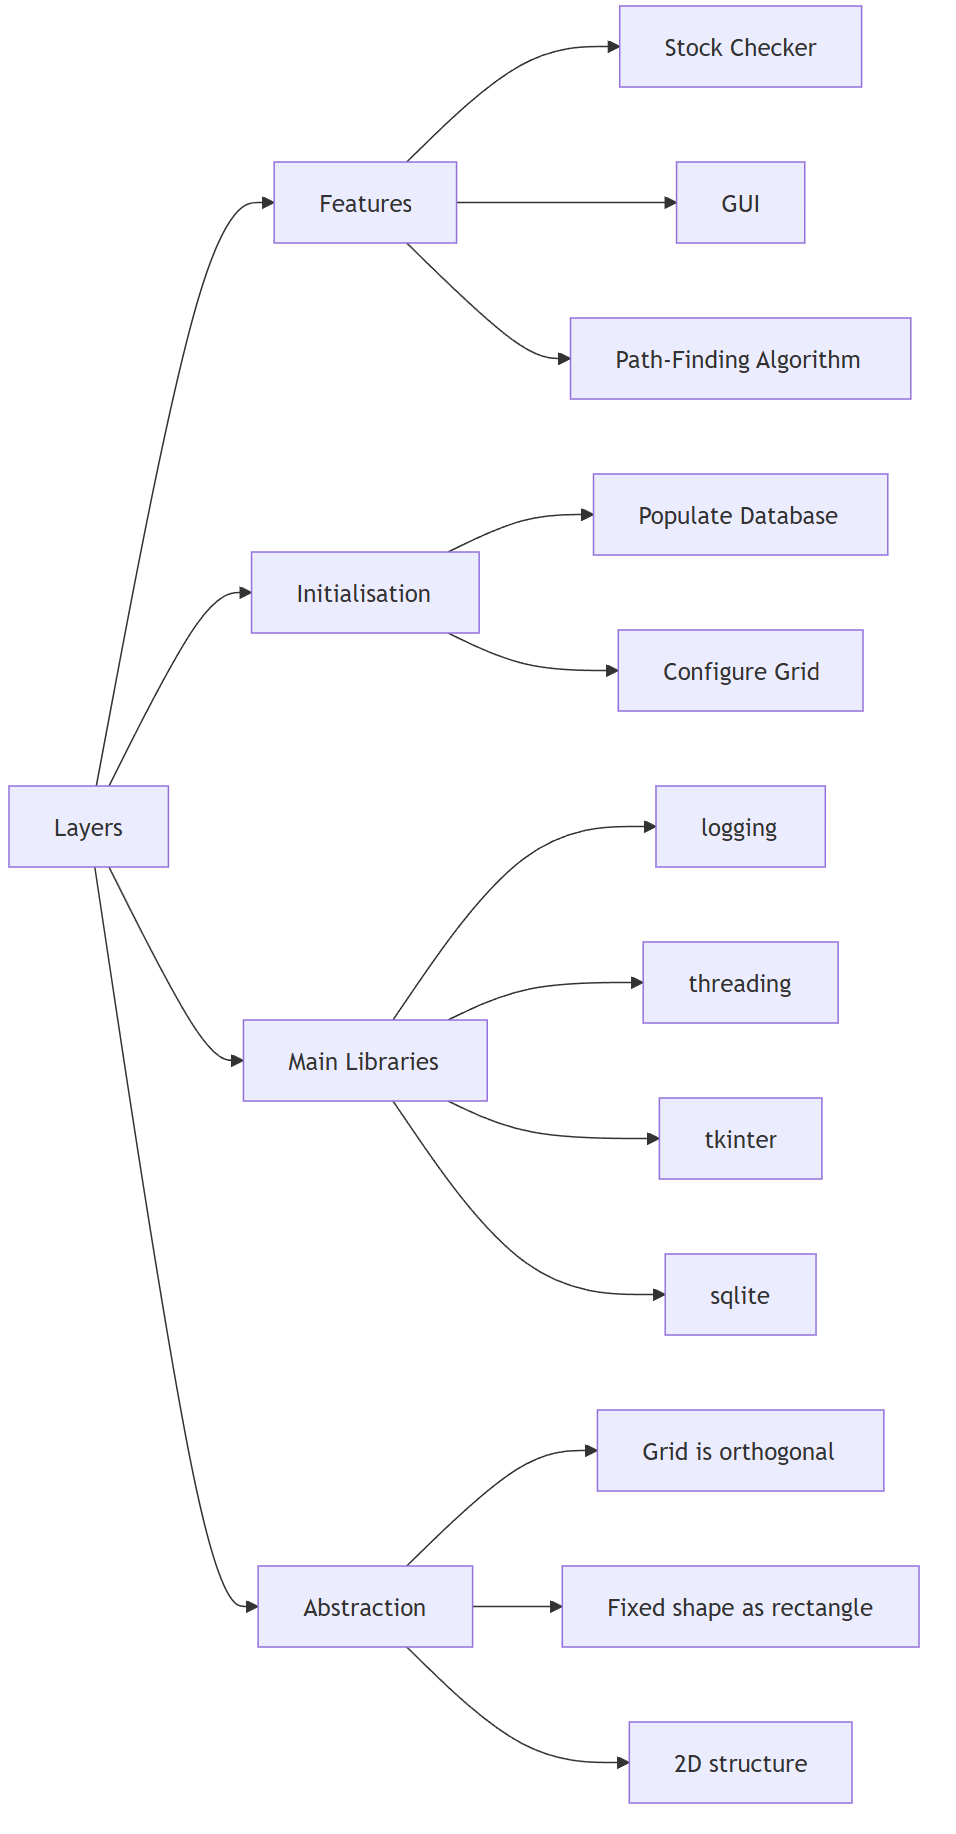
\includegraphics[width=0.5\linewidth]{Images/breakdown1.png}
	\caption{A further breakdown/structure of the pathfinding feature}
\end{figure}

\section{An initial breakdown of my solution}

Due to the complexity of my solution, I have decomposed my problem down into the fundamentals I believe will benefit me when designing a computational approach to this problem. I have broken down my complex solution into the initial layers of my design outline, and written justifications for each decision. See previous page for the chart outlining the basics.

\begin{enumerate}
    \item Features - this is the central part of the program - what will my program be able to do?
    \item Initialisation and Startup - this is how the program will configure itself - what must happen for my program to begin functioning?
    \item Main Libraries - this is how I will achieve the creation of this program - what is required to make my idea a reality?
    \item Abstraction - this is how I will break down the problem into more manageable chunks appropriate for a computational approach - how can I simplify the program and remove anything unnecessary?
\end{enumerate}


\subsection{Features}
This layer outlines the central features that the system offers in order for my client to benefit from this solution. This allows me to tackle each feature at a time, building a functional solution a section at a time.


\begin{itemize}
    \item Stock Checker - check whether an item is available before fetching it.
    \item Shortest Path Algorithm - find the fastest route to pick up all items
    \item GUI - make my solution more user-friendly and interactive
    \item Direct feedback to user - keep the user informed on what is happening, such as what path is being traced, what items are out of stock and so on.
\end{itemize}

See section x.x.x for a detailed explanation of these features, and see the next few pages for a basic outline of a further breakdown.

\newpage

\begin{figure}[!htbp]
	\centering
	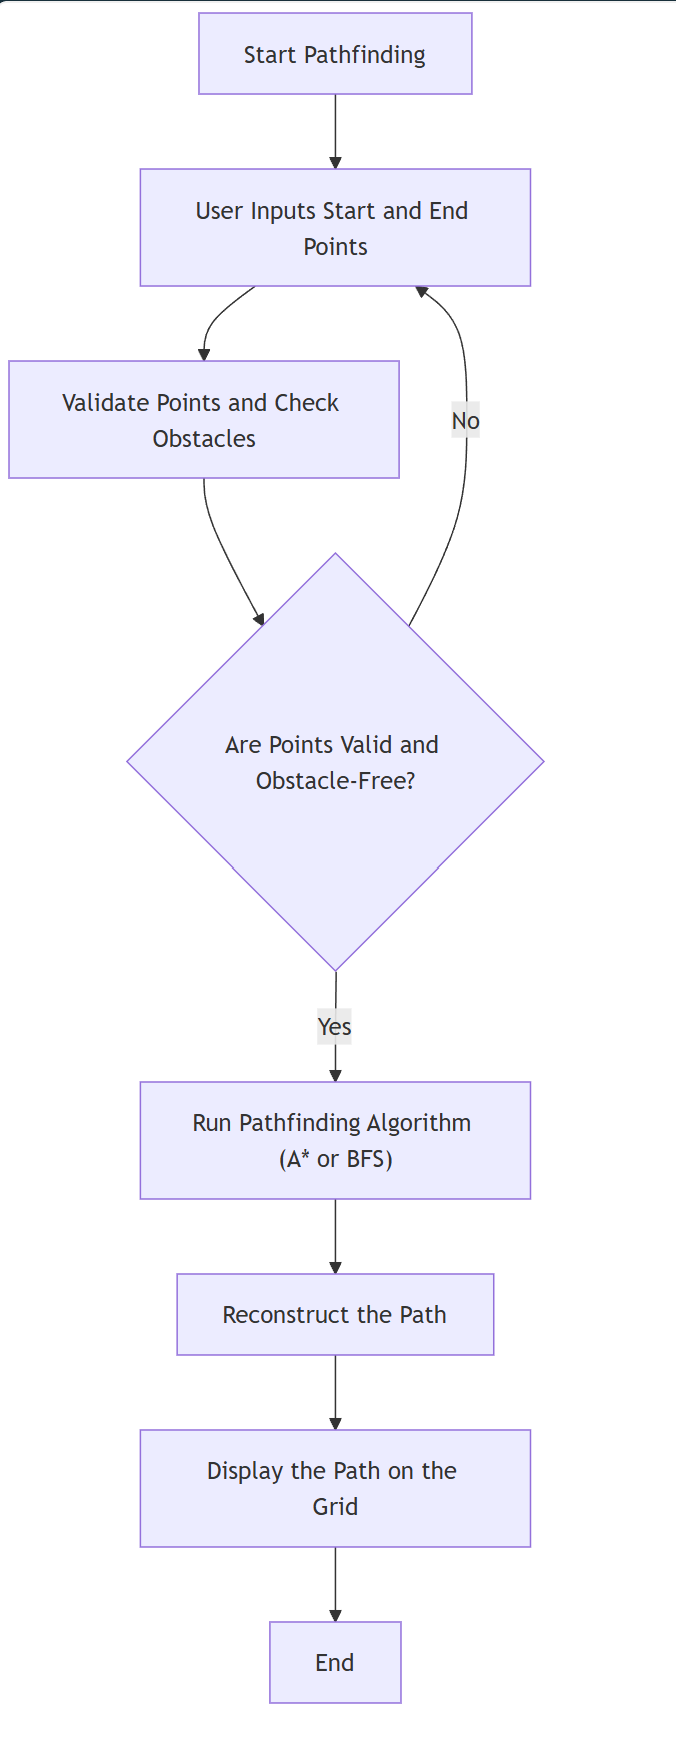
\includegraphics[width=0.5\linewidth]{Images/pfoutline.png}
	\caption{A further breakdown/structure of the pathfinding feature}
\end{figure}

\begin{figure}[!htbp]
	\centering
	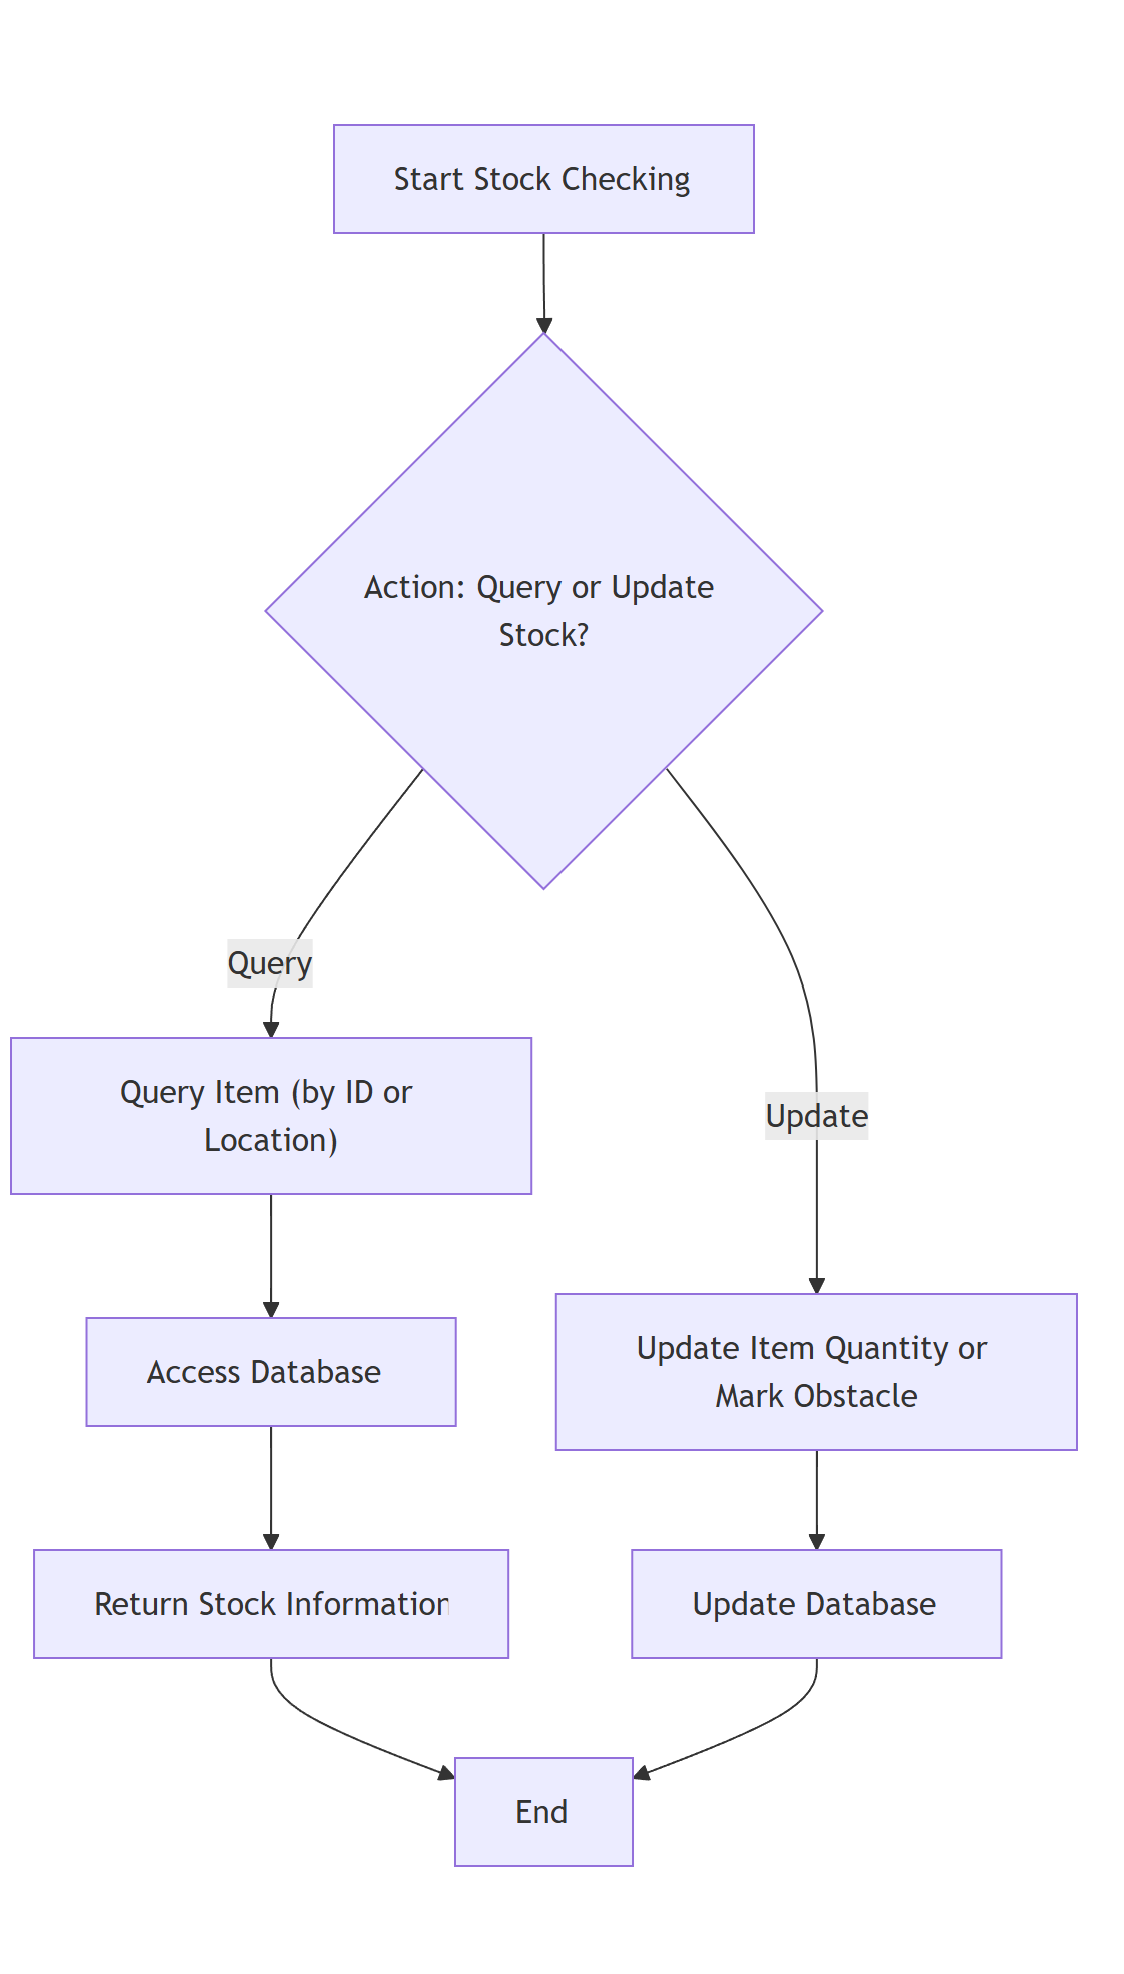
\includegraphics[width=0.9\linewidth]{Images/scoutline.png}
	\caption{A further breakdown/structure of the stock-checking feature}
\end{figure}

\begin{figure}[!htbp]
	\centering
	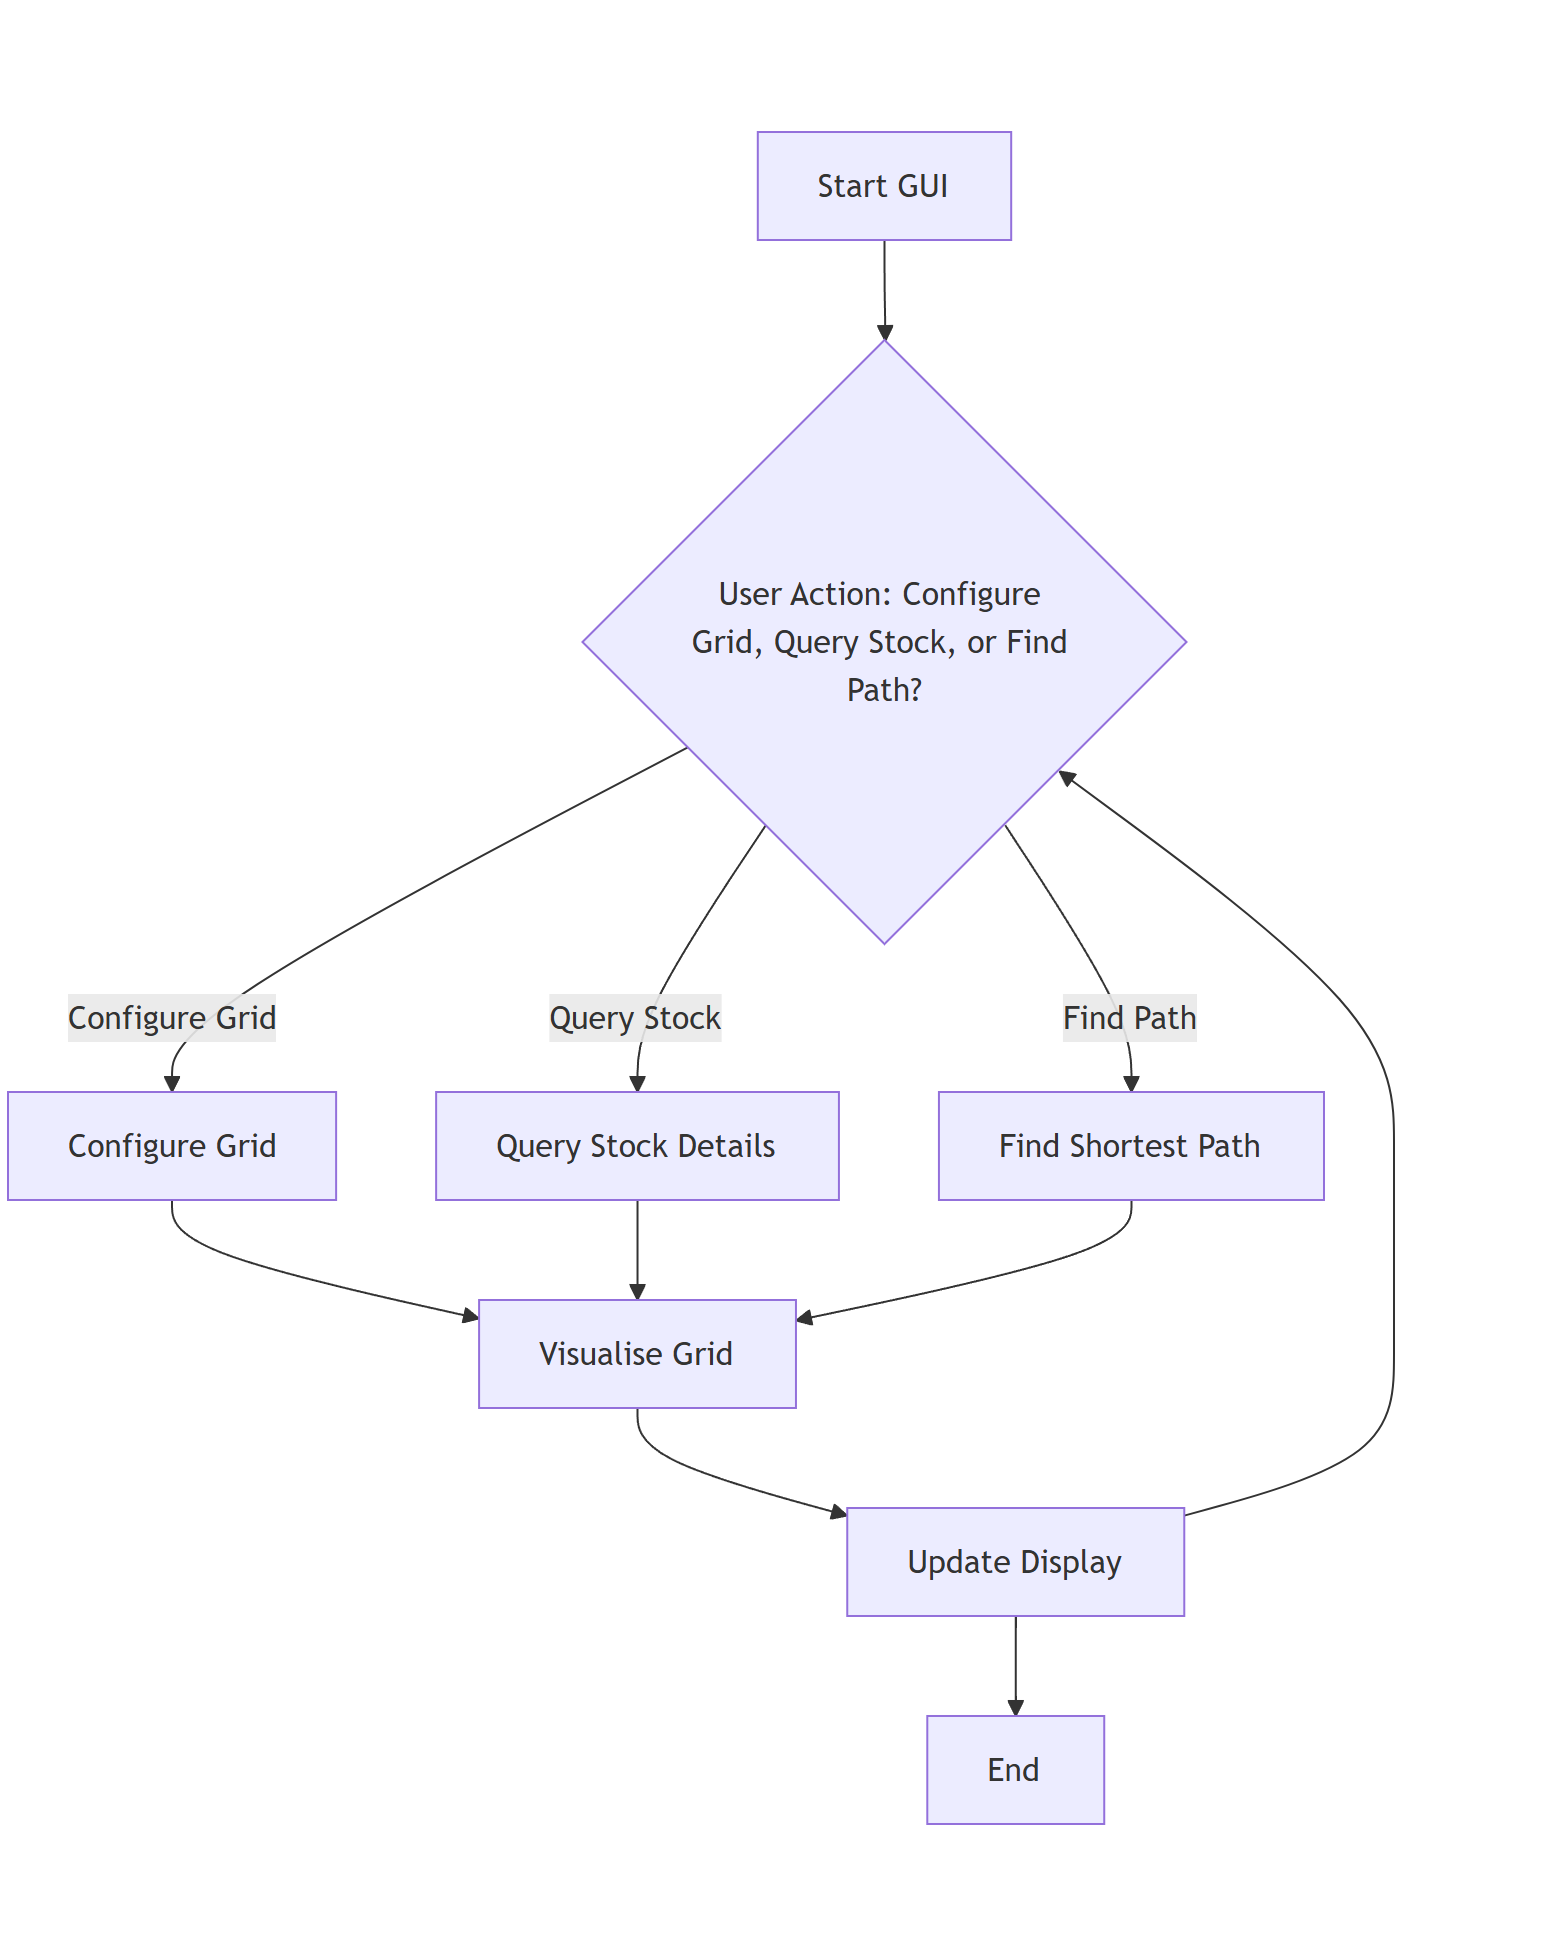
\includegraphics[width=1\linewidth]{Images/guioutline.png}
	\caption{A further breakdown/structure of the GUI}
\end{figure}


\newpage

\subsection{Initialisation and Startup}

This layer details the steps that will be involved in setting up and starting the system. This includes tasks like initialising the grid, ensuring the database exists and contains values, checking the shortest path algorithm, and displaying all elements of the GUI correctly.

\subsubsection{Setup of environment}

One objective is to configure the program initially - setting up the warehouse environment. It should be decomposed into the following:

\begin{itemize}
    \item Defining the rows and columns: As my program is designed to be used in a typical warehouse environment (one that is comprised of a grid structure), the user should input their warehouse specifications in the form of rows and columns.

    \item Initialise the database: Based on the number of rows and columns, an ID should be assigned to each square as an item to serve as a hypothetical product. The initial quantity should be randomised, then modified by the user.

    \item Load the interface: create all elements of the interface ready for user interaction: this should be done quite quickly.

\end{itemize} 

\subsubsection{Graphical User Interface}

Another objective is to create a functioning and responsive GUI with the following characteristics:

\begin{itemize}
    \item Responsive - The interface should be responsive to the user's clicks/presses and should update in an appropriate amount of time (e.g. 750ms) to display new content.

    \item Functional - The interface should allow users to access all features at the press of a button. The GUI will display key elements, including simple buttons to launch any subprogram of the solution such as a query system. It will also be a legend for the meanings of certain aspects of the visualisation of the warehouse, such as red for out-of-stock, green for the path, etc.

    \item Easy to use - The interface should be very simple and accessible to all users. The layout will be designed with simplicity and intuitiveness in mind, using a logical arrangement of buttons and visual elements. Tooltips and a help toolbar will be integrated to help users understand each feature without requiring detailed training.


\end{itemize}

See sections x.x.x for a prospective GUI

\newpage

\subsection{Main Libraries}

This layer lists the underlying software libraries or tools that are used to build the solution; these libraries provide the building blocks for each feature. Some examples of libraries include:
\begin{itemize}
    \item SQLite: This is a database management system that is used to store and manage data. In this case, I will be using it to store the warehouse layout, item IDs and quantities, as well as a boolean/binary property for whether a coordinate is an obstacle or not.
    \item Tkinter: This is Python's de-facto standard GUI package. It is a thin object-oriented layer on top of Tcl/Tk. Tkinter will be used to construct the GUI due to its simplicity and compatibility with Python. I will specifically using the 'grid' display sub-manager to create each aspect of the interface - this is due to the greater control it offers over positioning.
    \item Threading: This library is used to run multiple threads concurrently within a single process. Threads allow for parallel execution of tasks, enabling efficient utilization of system resources and the ability to perform multiple operations simultaneously. In my case, my algorithm is complex, requiring a large amount of processing power; threading allows the algorithm to run efficiently on the device by not restricting all processes like the GUI and database functions to run on a single thread - separating the algorithm will improve performance.
    \item Logging: This is fairly self-explanatory - the logging library is a built-in module used for generating and managing log messages. It provides a flexible framework for tracking events, debugging, and recording errors in a standardized and structured manner. I plan to use this to instrument my code - this will allow users to see exactly what is happening behind the GUI and allows me to target and debug any issues that may arise.

\end{itemize}

\subsection{Abstraction}

This layer outlines how I have simplified the solution down to essential components that need to be implemented - this is because some contextual parts of the solution are not necessary to craft a prototype and solution, as is the nature of abstraction. For example, current implementations use complex database systems to continually update and handle more advanced cases - since my implementation is designed to be scalable for smaller warehouses and businesses, some features can be abstracted, such as constant database updates and more complex elements of the database.


\subsection{Summary/Justifications}

Using the computational methods/principles, I felt it was best to split my solution into these layers, then further into what may be required to implement each section of the solution. By breaking it down like this, I can easily focus my efforts on a single part of my solution and then not have to worry in the future. Especially with OOP, this structure means I can easily diagnose and fix any errors that occur, while still leaving my code maintainable and clear. See the next page for the structure of my solution modelled as a top-down systems diagram and a class diagram so interactions between components are clear.

\newpage


\begin{figure}[!htbp]
    \centering
    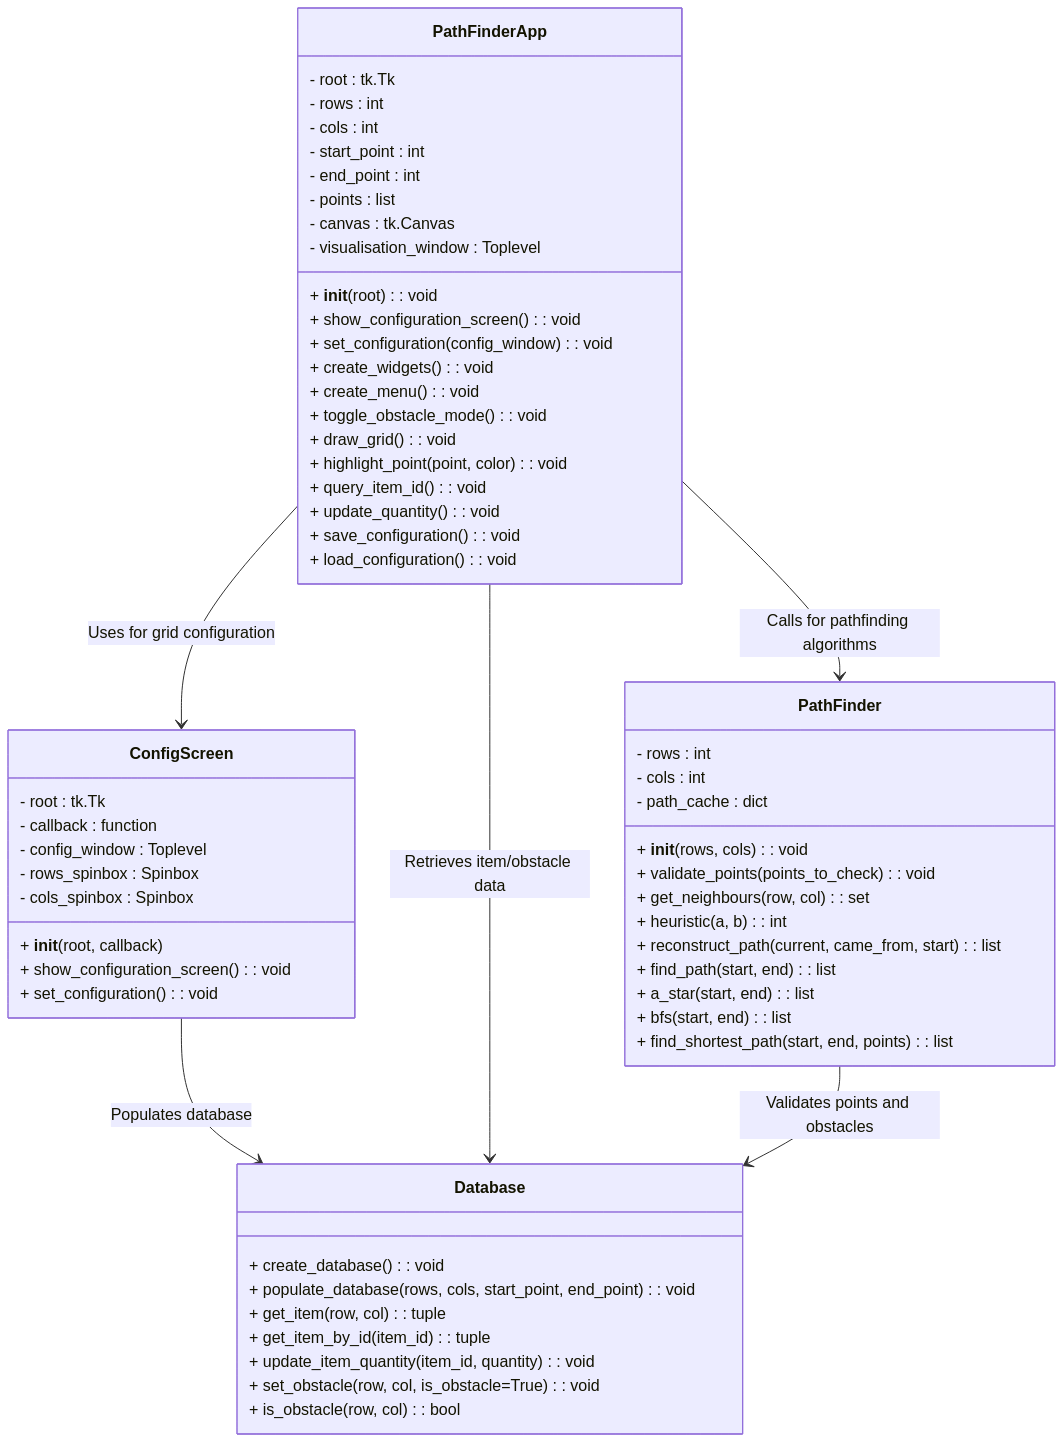
\includegraphics[width=1\linewidth]{Images/classdiag1.png}
    \caption{A hypothetical structure of my solution as a class diagram}
\end{figure}

\newpage

\begin{figure}[!htbp]
	\centering
	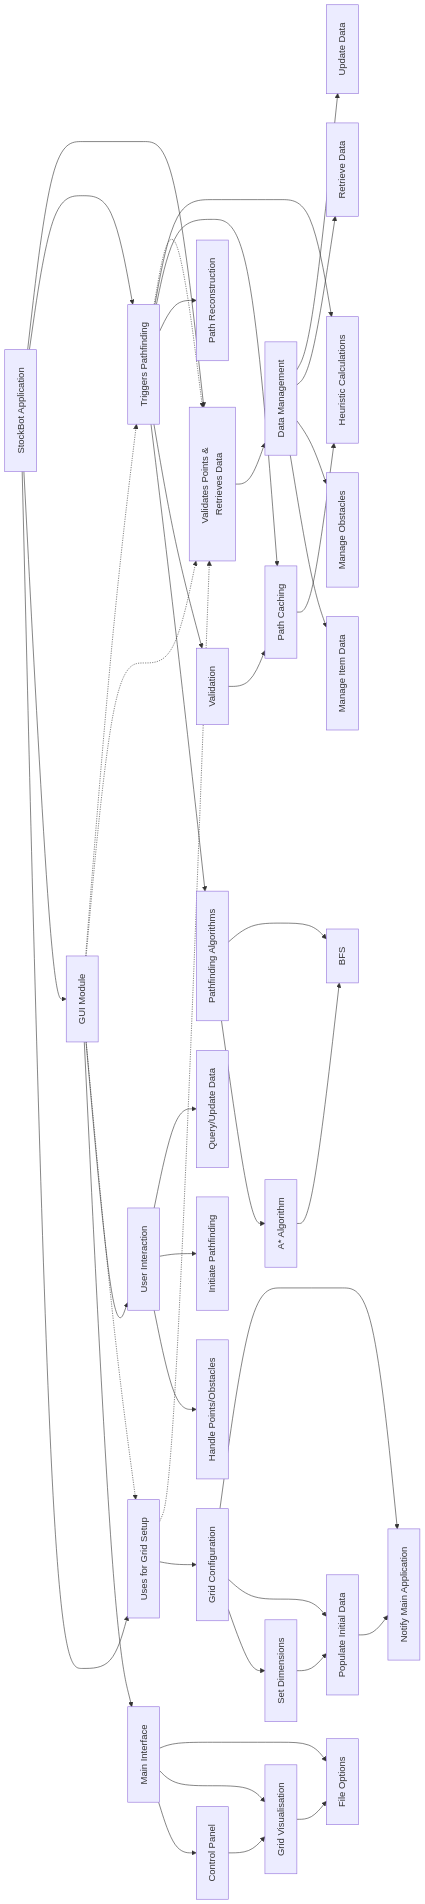
\includegraphics[width=0.3\linewidth]{Images/top-down-diagram.png}
	\caption{A basic top-down system diagram}
\end{figure}


\newpage
\section{Algorithm prototyping}

From the design outline, I will break down each section into the following subsections to begin prototyping my solution using a mixture of pseudocode and flowcharts:

\begin{enumerate}
    \item Create the primary shortest path algorithm (BFS).
    \item Build a rudimentary GUI complementing the SPA.
    \item Implement the database operations and the stock checker.
    \item Unify all the algorithms into a single prototype. (separate section)
\end{enumerate}

Once a fundamental program has been established, I will then proceed to do the following:

\begin{enumerate}
    \item Refine the algorithm to improve performance.
    \item Refine the GUI and add a visualisation of the path for ease of use and accessibility.
    \item Add help sections and more sophisticated database operations to improve user experience.
\end{enumerate}

\subsection{Creating the shortest path algorithm - BFS}

A good starting point is the central feature of this program: the shortest path algorithm. As my solution depends on this feature to outperform a human counterpart, it seems like a sensible point to start. I plan to implement a breadth-first search for the initial program, as it offers easy implementation, albeit at the cost of an optimum route - I can refine this later on as I am taking an object-oriented approach; I will separate the program into its respective features and place them in different files and classes, then call the required methods in a central file.

\begin{figure}[!htbp]
    \centering
    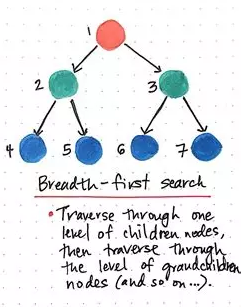
\includegraphics[width=0.35\linewidth]{Images/bfsvdfs.png}
    \caption{- BFS demonstration \cite{bfsimg}}
\end{figure}

\newpage

\subsubsection{BFS Flowchart}

\begin{figure}[!htbp]
    \centering
    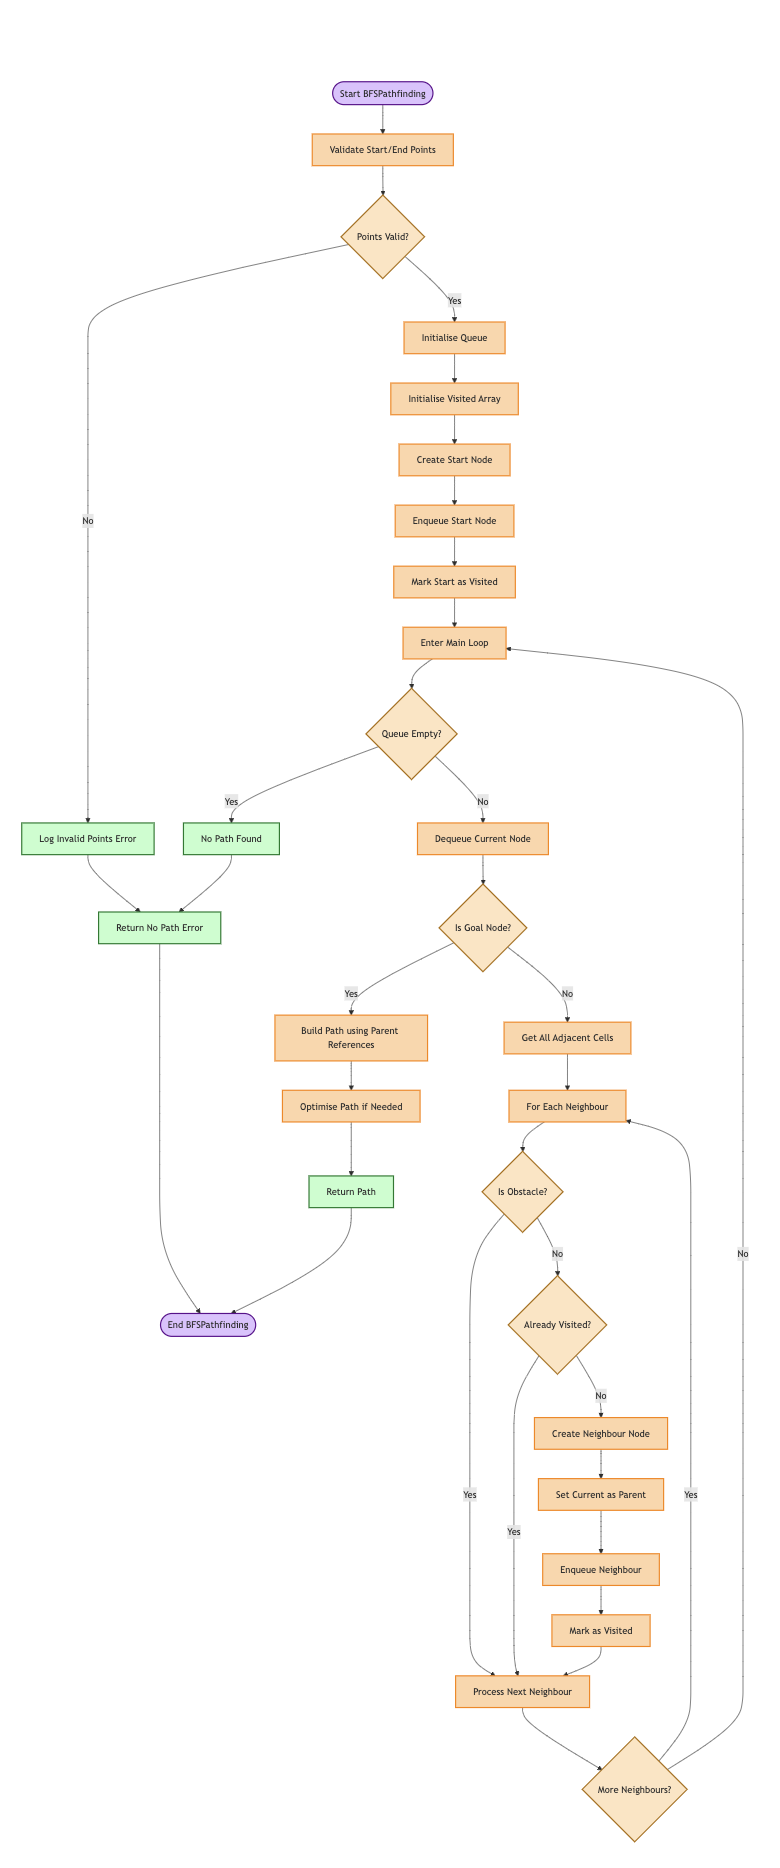
\includegraphics[width=0.56\linewidth]{Flowcharts/BFS2.png}
\end{figure}

\newpage


\subsubsection*{Grid Class}
The Grid class serves as a spatial abstraction layer that encapsulates the environment representation. This separation of concerns follows sound object-oriented principles by isolating the terrain data structure from the pathfinding algorithm. This approach enables independent modification of the environment's implementation without affecting the pathfinding logic, supporting the open-closed principle and enhancing maintainability.

\begin{itemize}
  \item \textbf{initialiseGrid}: Creates the initial grid structure with empty cells.
    \begin{itemize}
      \item \textit{Justification}: Critical foundation method that establishes the environment's structure. Without proper initialisation, the entire pathfinding process would have no valid space to operate in.
      \item \textit{Variables}: width: integer, height: integer, grid: 2D array
      \item \textit{Type Justification}: Integers provide precise dimensional control with minimal memory footprint. The 2D array structure provides O(1) access time to any cell using coordinates.
    \end{itemize}
    
  \item \textbf{isWithinBounds}: See Validation Functions section.
  
  \item \textbf{isObstacle}: See Validation Functions section.
  
  \item \textbf{getNeighbours}: Returns all traversable adjacent cells.
    \begin{itemize}
      \item \textit{Justification}: Core traversal method that implements the graph connectivity model. By defining neighbours in the cardinal directions, this method establishes the movement rules for the entire pathfinding system.
      \item \textit{Variables}: x: integer, y: integer, neighbours: array
      \item \textit{Type Justification}: Integer coordinates allow precise adjacency calculations. The returned array of position pairs provides a clean interface for iteration.
    \end{itemize}
  
  \item \textbf{setObstacle}: Sets a cell's obstacle status.
    \begin{itemize}
      \item \textit{Justification}: Provides essential mutability to the environment, allowing for dynamic map changes, responsive obstacles, or initial map setup.
      \item \textit{Variables}: x: integer, y: integer, isObstacle: boolean, grid[y][x]: boolean
      \item \textit{Type Justification}: Integer coordinates locate the target cell. The boolean parameter explicitly defines the intended state, preventing type coercion issues.
    \end{itemize}
\end{itemize}

\newpage

\subsubsection*{Pathfinder Class}
The Pathfinder class encapsulates the complete BFS algorithm implementation, separating the pathfinding logic from the environmental representation. This design choice promotes modularity and follows the single responsibility principle by focusing solely on path discovery. The class structure allows for straightforward extension to other pathfinding algorithms (such as A* or Dijkstra's) without modifying the Grid class or dependent systems.

\begin{itemize}
  \item \textbf{findPath}: Main BFS implementation to discover path.
    \begin{itemize}
      \item \textit{Justification}: The algorithmic core that translates the abstract BFS concept into executable code. This method orchestrates the entire search process, managing the queue, tracking visited states, and coordinating the exploration of the search space.
      \item \textit{Variables}: startX: integer, startY: integer, endX: integer, endY: integer, queue: array, visited: set
      \item \textit{Type Justification}: Integer coordinates provide precise position specification. Array implementation for the queue ensures FIFO ordering critical to BFS correctness. Set for visited tracking provides O(1) lookup time.
    \end{itemize}
    
  \item \textbf{validatePoints}: See Validation Functions section.
  
  \item \textbf{createNode}: Creates node objects with parent references.
    \begin{itemize}
      \item \textit{Justification}: Architectural keystone that establishes the parent-child relationships essential for path reconstruction. This method standardises the node structure throughout the algorithm.
      \item \textit{Variables}: x: integer, y: integer, parent: object or null, node: object
      \item \textit{Type Justification}: Integer coordinates locate the node in space. The recursive object structure creates a linked list that captures the entire path history.
    \end{itemize}
    
  \item \textbf{buildPath}: Reconstructs the path from goal to start.
    \begin{itemize}
      \item \textit{Justification}: Translation layer that converts the linked node structure into a usable, ordered path representation. Without this method, the algorithm would find the goal but be unable to report the actual path.
      \item \textit{Variables}: endNode: object, path: array
      \item \textit{Type Justification}: Node object with its chain of parent references contains the complete solution information, allowing backward path reconstruction.
    \end{itemize}
    
  \item \textbf{optimisePath}: Potential optimisation of the raw path.
    \begin{itemize}
      \item \textit{Justification}: Enhancement method that prepares for future expansion. While BFS provides the shortest path in terms of steps, real applications often benefit from smoothing, diagonal shortcuts, or other optimisations.
      \item \textit{Variables}: path: array, optimisedPath: array
      \item \textit{Type Justification}: Array of coordinate pairs offers sequential access and modification capabilities needed for path transformation algorithms.
    \end{itemize}
    
  \item \textbf{logError}: Reports pathfinding errors.
    \begin{itemize}
      \item \textit{Justification}: Diagnostic interface that improves debuggability and user feedback. Instead of silently failing or throwing exceptions, this method provides structured error reporting.
      \item \textit{Variables}: message: string, errorType: enum
      \item \textit{Type Justification}: String type provides flexible, human-readable error descriptions. The error type enumeration allows for programmatic handling of different error categories.
    \end{itemize}
\end{itemize}

\subsubsection*{Validation Functions}
Validation functions are critical components that ensure the integrity and correctness of the pathfinding process. They act as gatekeepers that prevent algorithm failure, detect impossible scenarios early, and provide meaningful feedback when errors occur. These functions collectively create a robust system that fails gracefully and provides useful diagnostic information.

\begin{itemize}
  \item \textbf{isWithinBounds} (Grid): Checks if coordinates are within grid boundaries.
    \begin{itemize}
      \item \textit{Justification}: Fundamental safety mechanism that prevents array index out-of-bounds errors which would crash the application. This method acts as a gatekeeper for all grid operations.
      \item \textit{Variables}: x: integer, y: integer, width: integer, height: integer
      \item \textit{Type Justification}: Integer coordinates allow for direct comparison operations against dimensions. Using the same integer type for all spatial values ensures consistent boundary checks.
    \end{itemize}
    
  \item \textbf{isObstacle} (Grid): Determines if a cell contains an obstacle.
    \begin{itemize}
      \item \textit{Justification}: Essential for path viability assessment. Without obstacle detection, the algorithm would potentially generate invalid paths through impassable terrain.
      \item \textit{Variables}: x: integer, y: integer, grid[y][x]: boolean
      \item \textit{Type Justification}: Integer coordinates provide direct access to the specific cell. The boolean value in each grid cell provides an unambiguous obstacle status.
    \end{itemize}
    
  \item \textbf{validatePoints} (Pathfinder): Validates start and end points.
    \begin{itemize}
      \item \textit{Justification}: Crucial pre-execution safeguard that prevents wasted computation on impossible scenarios. By checking validity upfront, this method fails fast when given invalid inputs.
      \item \textit{Variables}: startX: integer, startY: integer, endX: integer, endY: integer
      \item \textit{Type Justification}: Integer coordinates enable direct validation against grid dimensions and obstacle status. Using primitive types simplifies validation logic with standard comparison operators.
    \end{itemize}
\end{itemize}

\subsubsection{Example pseudocode of functions}

\begin{verbatim}
// Class representing the grid environment
class Grid {
    // Properties
    private cells[][]       // 2D array representing the grid
    private width           // Width of the grid
    private height          // Height of the grid
    
    // Constructor
    constructor(width, height) {
        this.width = width
        this.height = height
        this.cells = initialiseGrid(width, height)
    }
    
    // initialise grid with empty cells
    private initialiseGrid(width, height) {
        // Create a grid of specified dimensions
        // Default cells are traversable (not obstacles)
        return new Array(height).fill().map(() => new Array(width).fill(false))
    }
    
    // Check if given coordinates are within grid boundaries
    public isWithinBounds(x, y) {
        return x >= 0 && x < this.width && y >= 0 && y < this.height
    }
    
    // Check if cell at (x,y) is an obstacle
    public isObstacle(x, y) {
        if (!this.isWithinBounds(x, y)) return true
        return this.cells[y][x]
    }
    
    // Set a cell as an obstacle
    public setObstacle(x, y, isObstacle) {
        if (this.isWithinBounds(x, y)) {
            this.cells[y][x] = isObstacle
        }
    }

    
    // Get all neighbours of a given position that are not obstacles
    public getneighbours(x, y) {
        const neighbours = []
        const directions = [
            {dx: 0, dy: -1},  // Up
            {dx: 1, dy: 0},   // Right
            {dx: 0, dy: 1},   // Down
            {dx: -1, dy: 0}   // Left
        ]
        
        for (const dir of directions) {
            const newX = x + dir.dx
            const newY = y + dir.dy
            
            if (!this.isObstacle(newX, newY)) {
                neighbours.push({x: newX, y: newY})
            }
        }
        
        return neighbours
    }
}

// Class implementing the BFS pathfinding algorithm
class Pathfinder {
    // Properties
    private grid            // Reference to the Grid object
    
    // Constructor
    constructor(grid) {
        this.grid = grid
    }
    
    // Find path using BFS
    public findPath(startX, startY, endX, endY) {
        // Validate start and end points
        if (!this.validatePoints(startX, startY, endX, endY)) {
            this.logError("Invalid start or end points")
            return null
        }

        
        // initialise queue, visited array, and nodes
        const queue = []
        const visited = {}
        const startNode = this.createNode(startX, startY, null)
        
        // Enqueue start node and mark as visited
        queue.push(startNode)
        visited[`${startX},${startY}`] = true
        
        // Main BFS loop
        while (queue.length > 0) {
            // Dequeue current node
            const currentNode = queue.shift()
            
            // Check if goal reached
            if (currentNode.x === endX && currentNode.y === endY) {
                return this.buildPath(currentNode)
            }
            
            // Get all neighbours
            const neighbours = this.grid.getneighbours(currentNode.x, currentNode.y)
            
            // Process each neighbour
            for (const neighbour of neighbours) {
                const key = `${neighbour.x},${neighbour.y}`
                
                // Skip if already visited
                if (visited[key]) continue
                
                // Create neighbour node and set parent
                const neighbourNode = this.createNode(
                neighbour.x, neighbour.y, currentNode)
                
                // Enqueue neighbour and mark as visited
                queue.push(neighbourNode)
                visited[key] = true
            }
        }
        // No path found
        this.logError("No path found")
        return null
    }
    // Validate start and end points
    private validatePoints(startX, startY, endX, endY) {
        // Check if points are within grid boundaries
        if (!this.grid.isWithinBounds(startX, startY) ||
        !this.grid.isWithinBounds(endX, endY)) {
            return false
        }
        
        // Check if points are not obstacles
        if (this.grid.isObstacle(startX, startY) || 
        this.grid.isObstacle(endX, endY)) {
            return false
        }
        
        return true
    }
    
    // Create a new node
    private createNode(x, y, parent) {
        return {
            x: x,
            y: y,
            parent: parent
        }
    }
    
    // Build path by traversing parent references
    private buildPath(endNode) {
        const path = []
        let currentNode = endNode
        
        // Traverse from end node to start node
        while (currentNode !== null) {
            path.unshift({x: currentNode.x, y: currentNode.y})
            currentNode = currentNode.parent
        }
    }
    // Log an error message
    private logError(message) {
        console.log("Error: " + message)
    }
}
\end{verbatim}

\newpage

\subsubsection{Class Structure}
The implementation consists of two classes:
\begin{enumerate}
    \item \textbf{Grid Class}: Manages the environment representation and spatial operations
    \item \textbf{Pathfinder Class}: Implements the BFS algorithm for finding the shortest path
\end{enumerate}

These are separated as they deal with 2 different areas of the solution, making debugging easier and making the code more readable, as functions are now grouped as methods under classes.

\subsubsection{Grid Class}
\begin{itemize}
    \item \textbf{Core Properties}:
    \begin{itemize}
        \item \texttt{cells[][]}: A 2D array representing traversable spaces and obstacles
        \item \texttt{width} and \texttt{height}: Define the dimensions of the grid
    \end{itemize}
    \item \textbf{Key Methods}:
    \begin{itemize}
        \item \texttt{isWithinBounds()}: Ensures coordinates remain within grid limits
        \item \texttt{isObstacle()}: Determines if a cell is blocked and cannot be traversed
        \item \texttt{getneighbours()}: Returns all adjacent traversable cells in orthogonal directions (Up, down, left, right)
    \end{itemize}
\end{itemize}

I used a 2D array as it is similar to a grid in most aspects, and is a good abstraction of a warehouse layout, as each element could represent a shelf/area in a warehouse. I passed width \& height as attributes as they are required to calculate start \& end points.

The \verb|isWithinBounds()| and \verb|isObstacle()| methods are used to validate points so that the program does not fail and is robust.

\subsubsection{Pathfinder Class}
\begin{itemize}
    \item \textbf{Core Methods}:
    \begin{itemize}
        \item \texttt{findPath()}: The main method that orchestrates the entire BFS process
        \item Uses a queue to ensure cells are visited in order of increasing distance from start (FIFO)
    \end{itemize}
    \item \textbf{Supporting Methods}:
    \begin{itemize}
        \item \texttt{validatePoints()}: Performs comprehensive validation of start and end coordinates
        \item \texttt{createNode()}: Constructs node objects with parent references for path reconstruction
        \item \texttt{buildPath()}: Reconstructs the complete path by traversing parent references backward
    \end{itemize}
\end{itemize}

The methods in this class are mostly self-explanatory. The \verb|findPath()| method is used to find a path between 2 points. The \verb|validatePoints()| method ensures the points are valid, using the \verb|grid| methods. The \verb|createNode()| and \verb|buildPath()| methods are used to backtrack and construct the actual path.

\newpage

\subsubsection{BFS Implementation Details}
\begin{enumerate}
    \item \textbf{Initialisation Phase}:
    \begin{itemize}
        \item Validates input points to ensure they're within bounds and not obstacles
        \item Sets up the queue with the starting node and marks it as visited
    \end{itemize}
    \item \textbf{Exploration Phase}:
    \begin{itemize}
        \item Processes nodes in breadth-first order (nearest nodes first)
        \item For each node, checks if it's the goal before exploring neighbours
        \item Avoids revisiting cells by maintaining a visited state dictionary
    \end{itemize}
    \item \textbf{Path Reconstruction Phase}:
    \begin{itemize}
        \item When the goal is found, traces back through parent references
        \item Builds the path from start to end in the correct order
    \end{itemize}
\end{enumerate}

\subsubsection{Validation Strategy}
\begin{itemize}
    \item \textbf{Input Validation}: Checks that start and end points are valid before beginning the search
    \item \textbf{Boundary Validation}: Prevents accessing cells outside the grid boundaries
    \item \textbf{Obstacle Validation}: Ensures only traversable cells are considered during pathfinding
    \item \textbf{Duplicate Prevention}: Avoids processing the same cell multiple times
\end{itemize}

\textbf{}\newline This is an example of how the BFS algorithm could be implemented in pseudocode. As my program grows in complexity, I will most likely deviate from this fixed template of classes but still maintain all the features. For example, when adding the A* algorithm, I can extract the validation features and have a single class dedicated to pathfinding operations only, while another class can handle validation.

\newpage

\subsection{Creating the shortest path algorithm - A*}

\begin{figure}[!htbp]
	\centering
	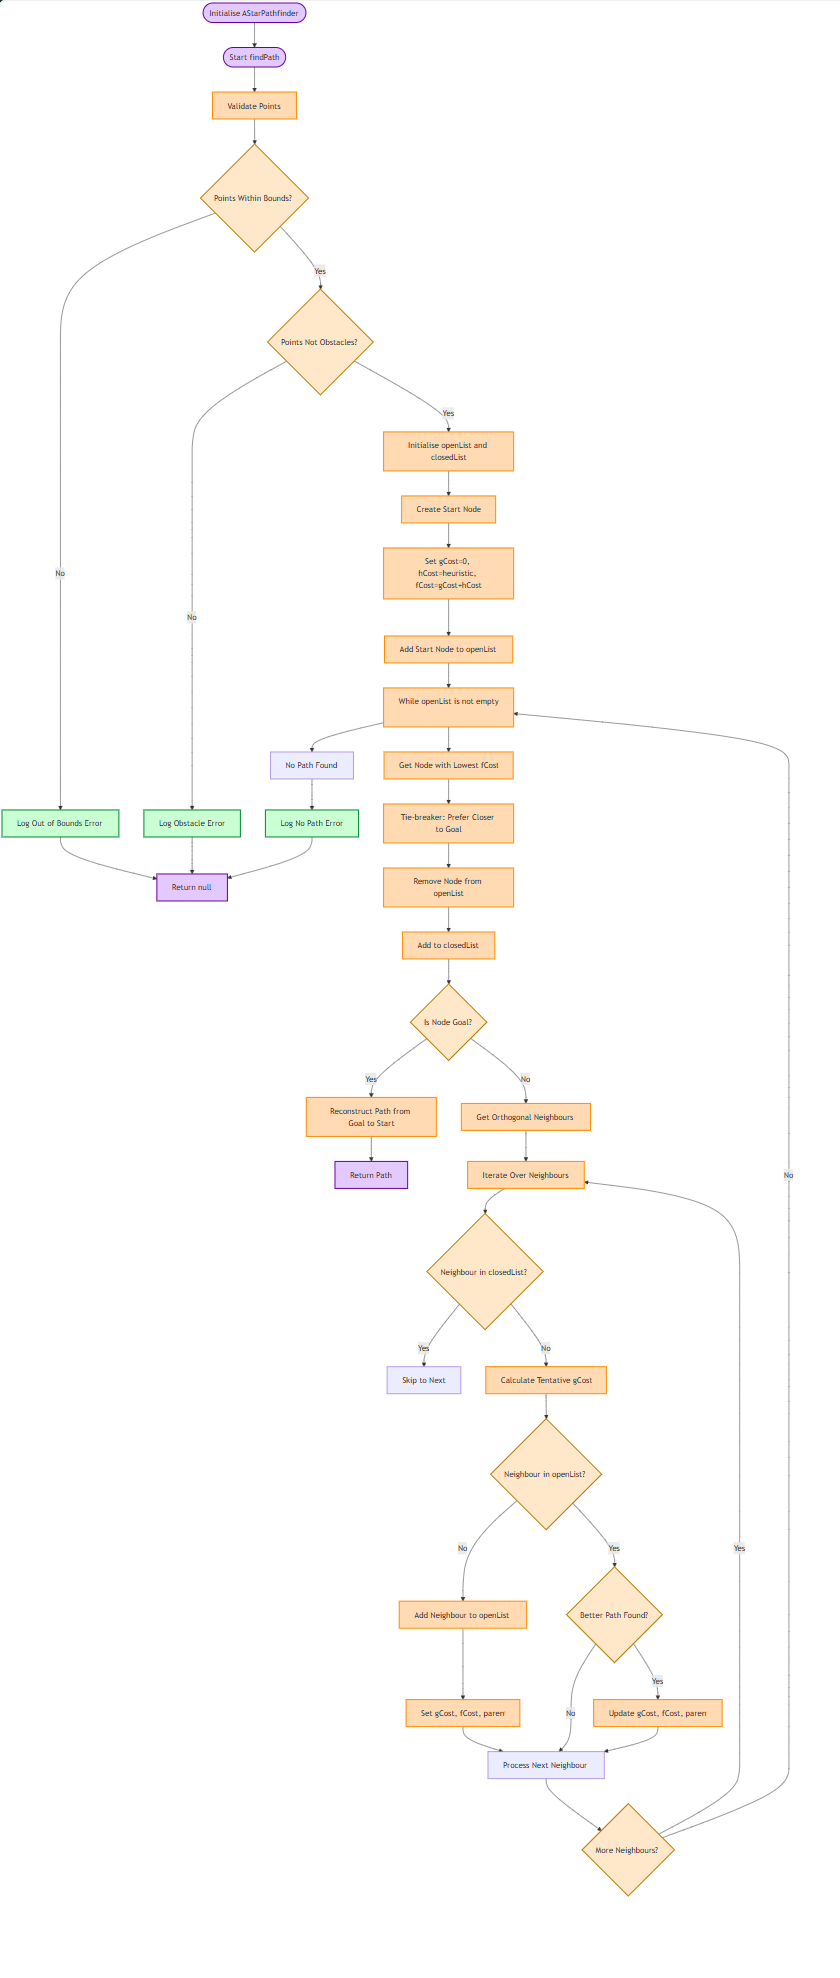
\includegraphics[width=0.55\linewidth]{Flowcharts/basicastar.png}
\end{figure}

\newpage

The A* algorithm is a refinement in my program, a step above BFS in terms of performance. While more complex to implement, it often finds the path faster as it incorporates a heuristic system.

\begin{itemize} \item \textbf{findPath}: Main A* implementation that orchestrates the pathfinding process. \begin{itemize} \item \textit{Justification}: Serves as the algorithmic controller that coordinates all aspects of the A* search, from initialisation through node exploration to final path construction. The method systematically explores the grid by always selecting the most promising nodes first, ensuring an optimal solution whilst minimising the search space. \item \textit{Variables}: startX: integer, startY: integer, endX: integer, endY: integer, openList: array, closedList: set \item \textit{Type Justification}: Integer coordinates provide precise position specification on the grid. The array implementation for openList is straightforward to manipulate, whilst the set data structure for closedList provides efficient lookup for previously explored nodes. \end{itemize}

\item \textbf{createNode}: Constructs node objects with cost values and parent references. \begin{itemize} \item \textit{Justification}: Standardises the node structure throughout the algorithm and encapsulates the creation of the node object that must track multiple cost values along with position and parentage. Centralising this construction ensures consistency across all node instances. \item \textit{Variables}: x: integer, y: integer, parent: object or null, gCost: integer, hCost: integer, fCost: integer \item \textit{Type Justification}: Integer coordinates identify spatial position on the grid. Integer cost values enable mathematical operations for comparative pathfinding whilst avoiding floating-point precision issues. The parent reference creates a linked structure essential for path reconstruction. \end{itemize}

\item \textbf{calculateHeuristic}: Estimates the distance from a node to the goal. \begin{itemize} \item \textit{Justification}: Provides the crucial admissible heuristic function that gives A* its efficiency advantage over algorithms like Dijkstra's. For orthogonal movement, the Manhattan distance perfectly estimates the minimum possible cost to reach the goal without overestimation, guiding exploration towards the target. \item \textit{Variables}: x: integer, y: integer, endX: integer, endY: integer \item \textit{Type Justification}: Integer coordinates allow for precise Manhattan distance calculation, which is the sum of horizontal and vertical distances, matching exactly the movement constraints of our orthogonal-only system. \end{itemize}

\item \textbf{getBestNode}: Finds the node with the lowest f-cost in the open list. \begin{itemize} \item \textit{Justification}: This method implements the greedy selection aspect of A* by ensuring that the most promising nodes are explored first. This prioritisation is fundamental to the algorithm's efficiency and optimality guarantees. \item \textit{Variables}: openList: array, bestNode: object \item \textit{Type Justification}: The array structure allows for iteration through all candidate nodes, whilst the node object provides access to the cost values needed for comparison. The tie-breaking mechanism using h-cost biases exploration toward the goal when f-costs are equal. \end{itemize}

\item \textbf{getOrthogonalNeighbours}: Returns valid adjacent nodes in the four cardinal directions. \begin{itemize} \item \textit{Justification}: Implements the graph connectivity model for a grid with orthogonal-only movement. By limiting movement to the four cardinal directions, this method enforces the movement constraints of our simplified pathfinding system. \item \textit{Variables}: x: integer, y: integer, directions: array, neighbours: array \item \textit{Type Justification}: Integer coordinates enable precise adjacency calculations. The array of direction vectors provides a clean way to represent and iterate through the four cardinal directions, whilst the resulting neighbours array offers a standard format for the main algorithm to process. \end{itemize}

\item \textbf{buildPath}: Reconstructs the path from goal to start using node parentage. \begin{itemize} \item \textit{Justification}: Transforms the linked structure of parent references into a usable, sequential path representation. This backward traversal efficiently constructs the optimal path once the goal is reached, without requiring separate bookkeeping during the search phase. \item \textit{Variables}: endNode: object, path: array, currentNode: object \item \textit{Type Justification}: The node object contains the complete solution through its parent chain. The resulting array provides a clean, ordered representation of waypoints that can be directly used by path-following systems. \end{itemize} \end{itemize}

\subsubsection*{Validation Functions}

These are identical to BFS validation.

\subsubsection{Example pseudocode for A*}

\begin{verbatim}
class AStarPathfinder:
    # Class variables
    grid: Grid            # Reference to Grid class for terrain information
    openList: Array       # Nodes to be evaluated, manually sorted by fCost
    closedList: Set       # Nodes already evaluated
    
    # Constructor
    function constructor(grid):
        this.grid = grid
    
    # Main pathfinding method
    function findPath(startX, startY, endX, endY):
        # Validate inputs
        if not this.validatePoints(startX, startY, endX, endY):
            this.logError("Invalid start or end point")
            return null
        
        # Initialise data structures
        this.openList = []
        this.closedList = new Set()
        
        # Create and add start node
        startNode = this.createNode(startX, startY, null)
        startNode.gCost = 0
        startNode.hCost = this.calculateHeuristic(startX, startY, endX, endY)
        startNode.fCost = startNode.gCost + startNode.hCost
        this.openList.push(startNode)
        
        # Main loop
        while this.openList.length > 0:
            # Get node with lowest fCost
            currentNode = this.getBestNode()
            
            # Check if goal reached
            if currentNode.x == endX and currentNode.y == endY:
                return this.buildPath(currentNode)
            
            # Remove current from open list and add to closed list
            this.openList.splice(this.openList.indexOf(currentNode), 1)
            this.closedList.add(currentNode.x + "," + currentNode.y)
            
            # Process all neighbours (only orthogonal: up, right, down, left)
            neighbours = this.getOrthogonalNeighbours(currentNode.x, currentNode.y)
            
            for each neighbour in neighbours:
                neighbourKey = neighbour.x + "," + neighbour.y
                
                # Skip nodes in closed list
                if this.closedList.has(neighbourKey):
                    continue
                
                # Each step costs 1 unit in this simplified version
                tentativeGCost = currentNode.gCost + 1
                
                # Check if this node is already in the open list
                existingNode = null
                for each node in this.openList:
                    if node.x == neighbour.x and node.y == neighbour.y:
                        existingNode = node
                        break
                
                if not existingNode:
                    # New node, add to open list
                    neighbourNode = this.createNode(
                    neighbour.x, neighbour.y, currentNode
                    )
                    neighbourNode.gCost = tentativeGCost
                    neighbourNode.hCost = this.calculateHeuristic(
                    neighbour.x, neighbour.y, endX, endY
                    )
                    neighbourNode.fCost = neighbourNode.gCost + neighbourNode.hCost
                    this.openList.push(neighbourNode)
                elif tentativeGCost < existingNode.gCost:
                    # Better path found, update existing node
                    existingNode.gCost = tentativeGCost
                    existingNode.fCost = tentativeGCost + existingNode.hCost
                    existingNode.parent = currentNode
                }
        }
        
        # No path found
        this.logError("No path exists between start and end points")
        return null
    
    # Create a node object with cost values
    function createNode(x, y, parent):
        return {
            x: x,
            y: y,
            gCost: 0,     # Cost from start to this node
            hCost: 0,     # Manhattan distance from this node to goal
            fCost: 0,     # Total cost (g + h)
            parent: parent # Reference to parent node for path reconstruction
        }
    
    # Calculate Manhattan distance from node to goal
    function calculateHeuristic(x, y, endX, endY):
        # Manhattan distance (absolute difference in x plus absolute difference in y)
        return abs(x - endX) + abs(y - endY)
    
    # Find node with lowest fCost in the open list
    function getBestNode():
        bestNode = this.openList[0]
        
        for each node in this.openList:
            if node.fCost < bestNode.fCost:
                bestNode = node
            # Tie-breaker: prefer nodes closer to the goal
            elif node.fCost == bestNode.fCost and node.hCost < bestNode.hCost:
                bestNode = node
        
        return bestNode
    
    # Get orthogonal neighbouring positions (up, right, down, left)
    function getOrthogonalNeighbours(x, y):
        neighbours = []
        
        # The four orthogonal directions
        directions = [
            {x: 0, y: -1},  # Up
            {x: 1, y: 0},   # Right
            {x: 0, y: 1},   # Down
            {x: -1, y: 0}   # Left
        ]
        
        for each dir in directions:
            newX = x + dir.x
            newY = y + dir.y
            
            # Check if position is valid (within bounds and not an obstacle)
            if this.grid.isWithinBounds(newX, newY) and not this.grid.isObstacle(newX, newY):
                neighbours.push({x: newX, y: newY})
        
        return neighbours
    
    # Reconstruct path from goal node to start node
    function buildPath(endNode):
        path = []
        currentNode = endNode
        
        # Traverse parent chain from end to start
        while currentNode:
            path.unshift([currentNode.x, currentNode.y])  # Add to front
            currentNode = currentNode.parent
        
        return path
    
    # Validate start and end points
    function validatePoints(startX, startY, endX, endY):
        # Check if points are within grid bounds
        if not this.grid.isWithinBounds(startX, startY) or not
        this.grid.isWithinBounds(endX, endY):
        
            return false
        
        # Check if points are not obstacles
        if this.grid.isObstacle(startX, startY) or this.grid.isObstacle(endX, endY):
            return false
        
        return true
    
    # Log errors for diagnostics
    function logError(message):
        console.log("AStarPathfinder Error: " + message)
\end{verbatim}

\newpage

\subsection{GUI Logic}

\begin{figure}[htbp]
	\centering
	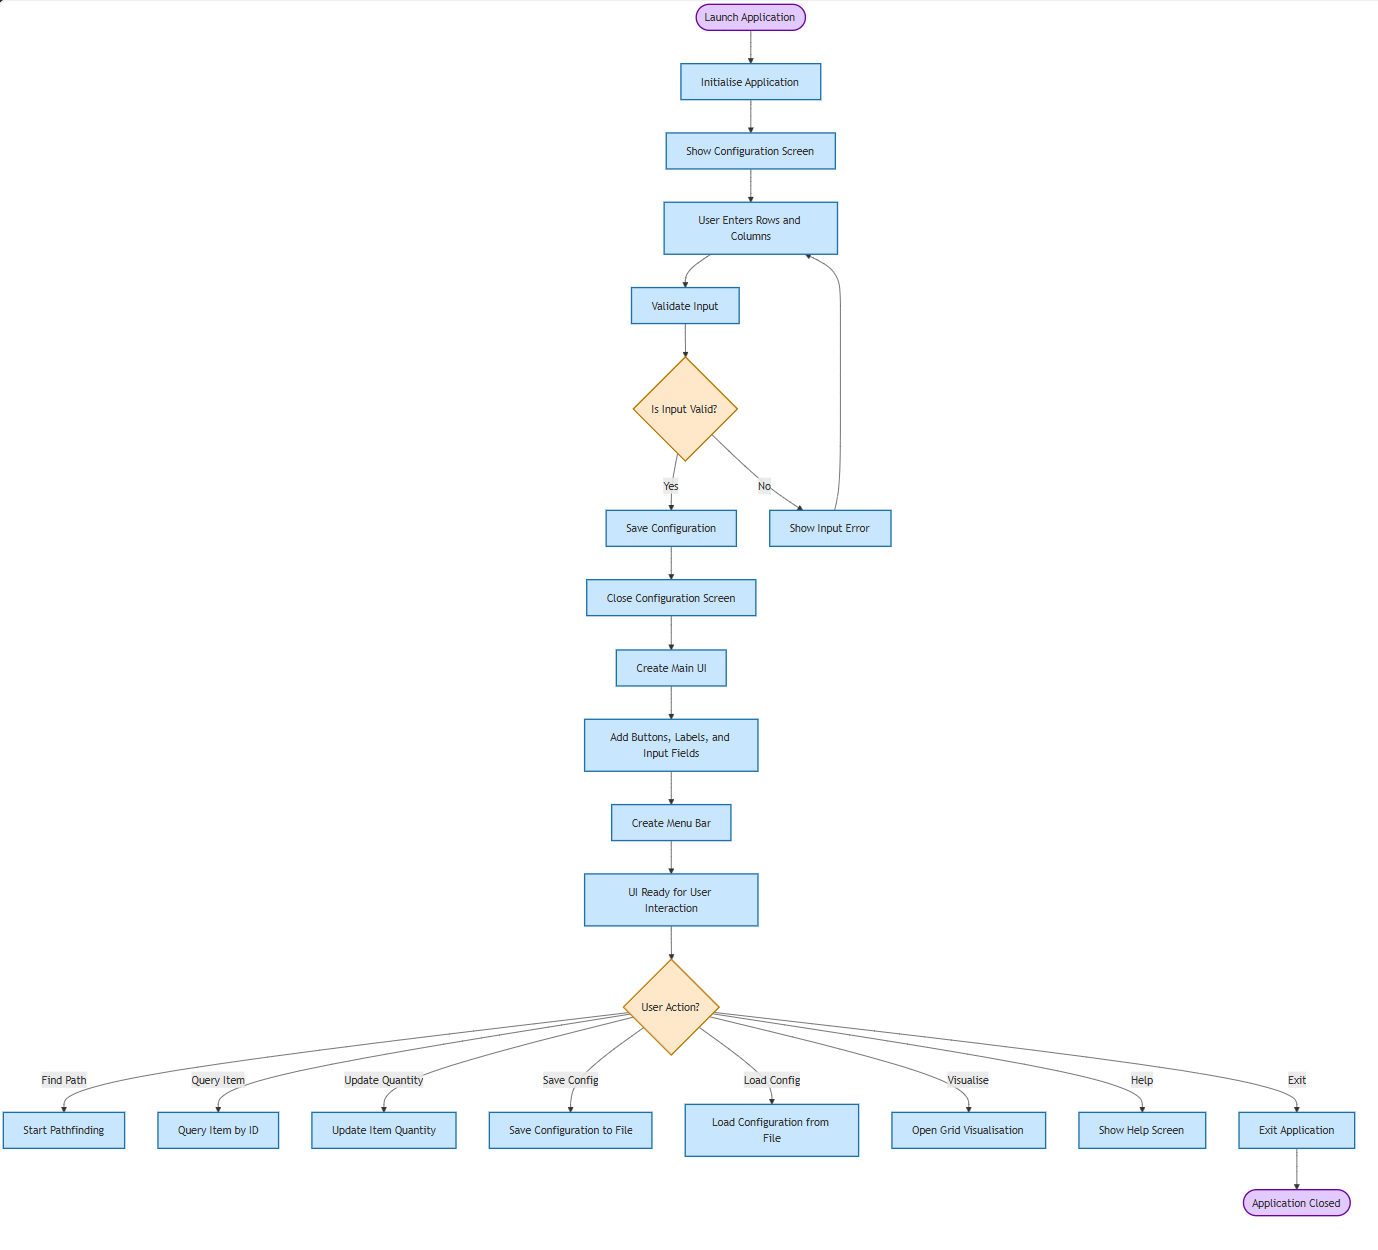
\includegraphics[width=1\linewidth]{Flowcharts/guiflowchart.png}
	
\end{figure}

\newpage

\subsection{Database operations}

\begin{figure}[htbp]
    \centering
    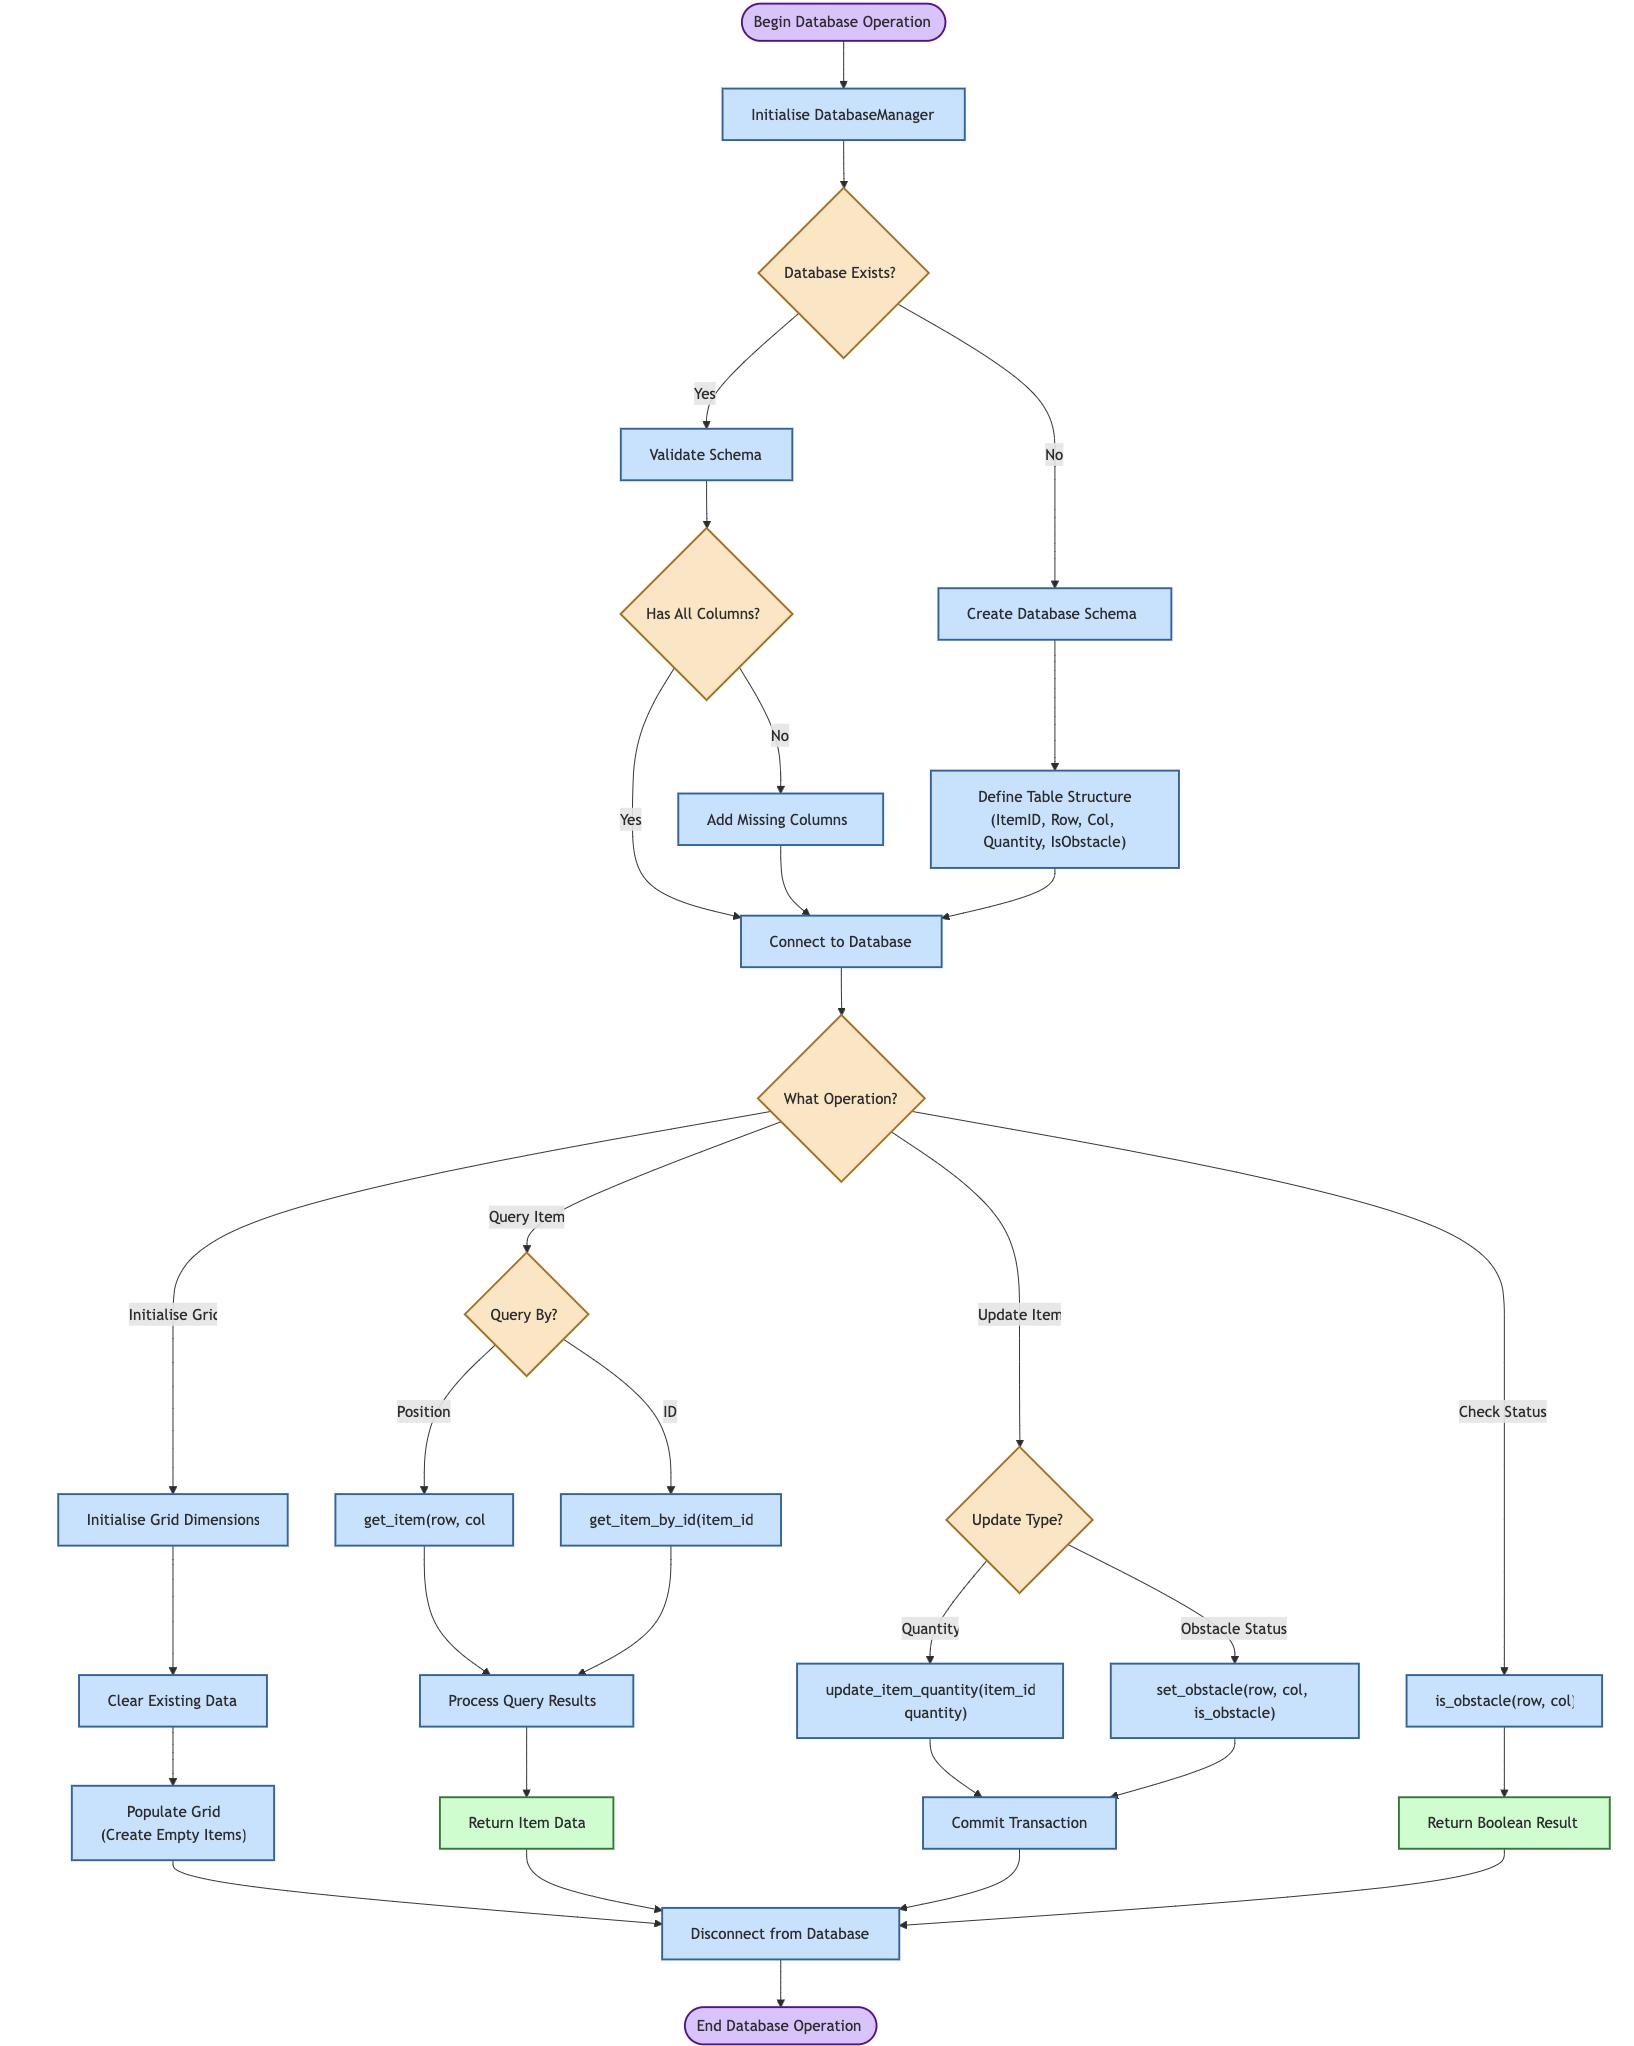
\includegraphics[width=0.91\linewidth]{Flowcharts/dbops1.png}

\end{figure}

\newpage

\subsubsection{Database validation}

\begin{figure}[htbp]
    \centering
    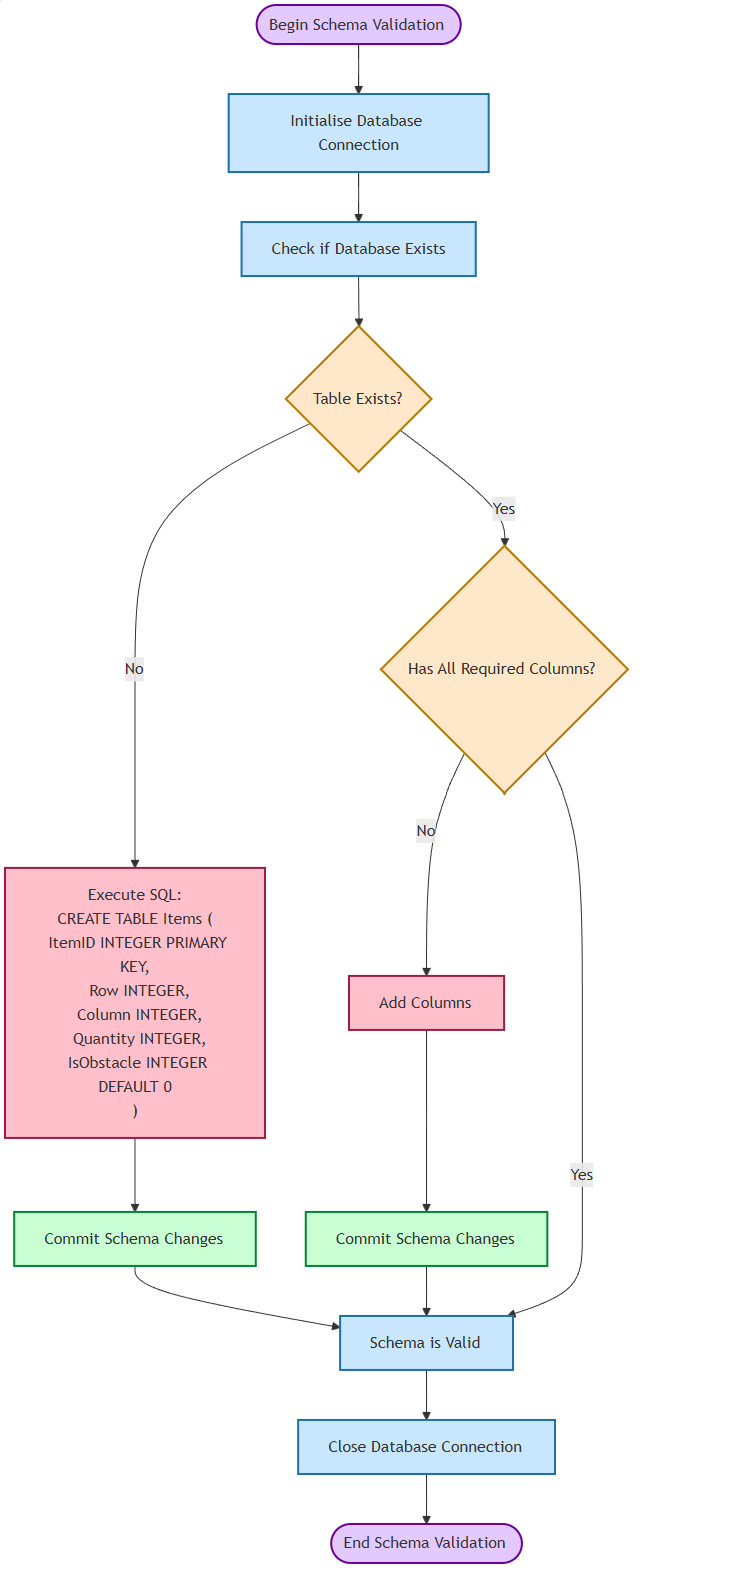
\includegraphics[width=1\linewidth]{Flowcharts/dbinit.png}
\end{figure}

\newpage

\subsubsection{Database query}

\begin{figure}[htbp]
    \centering
    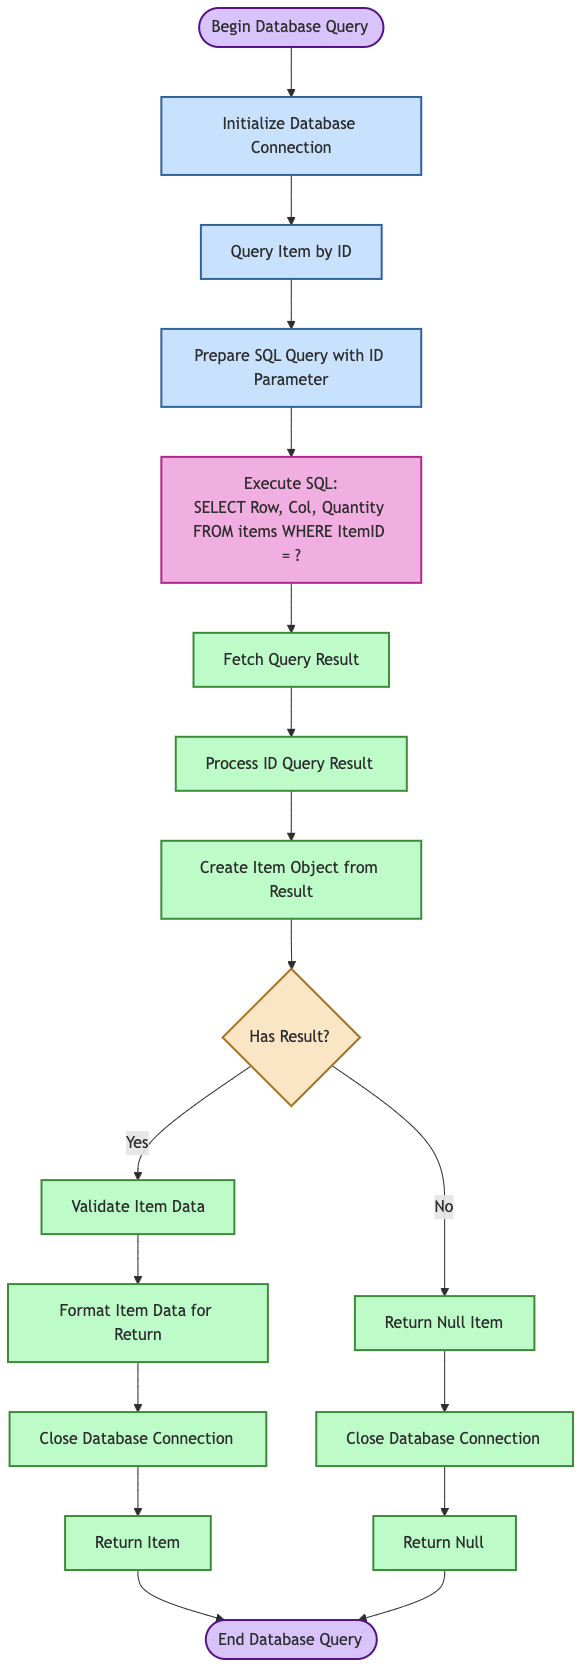
\includegraphics[width=0.4\linewidth]{Flowcharts/dbquery.png}
\end{figure}

\newpage

\subsubsection{Database update}

\begin{figure}[htbp]
    \centering
    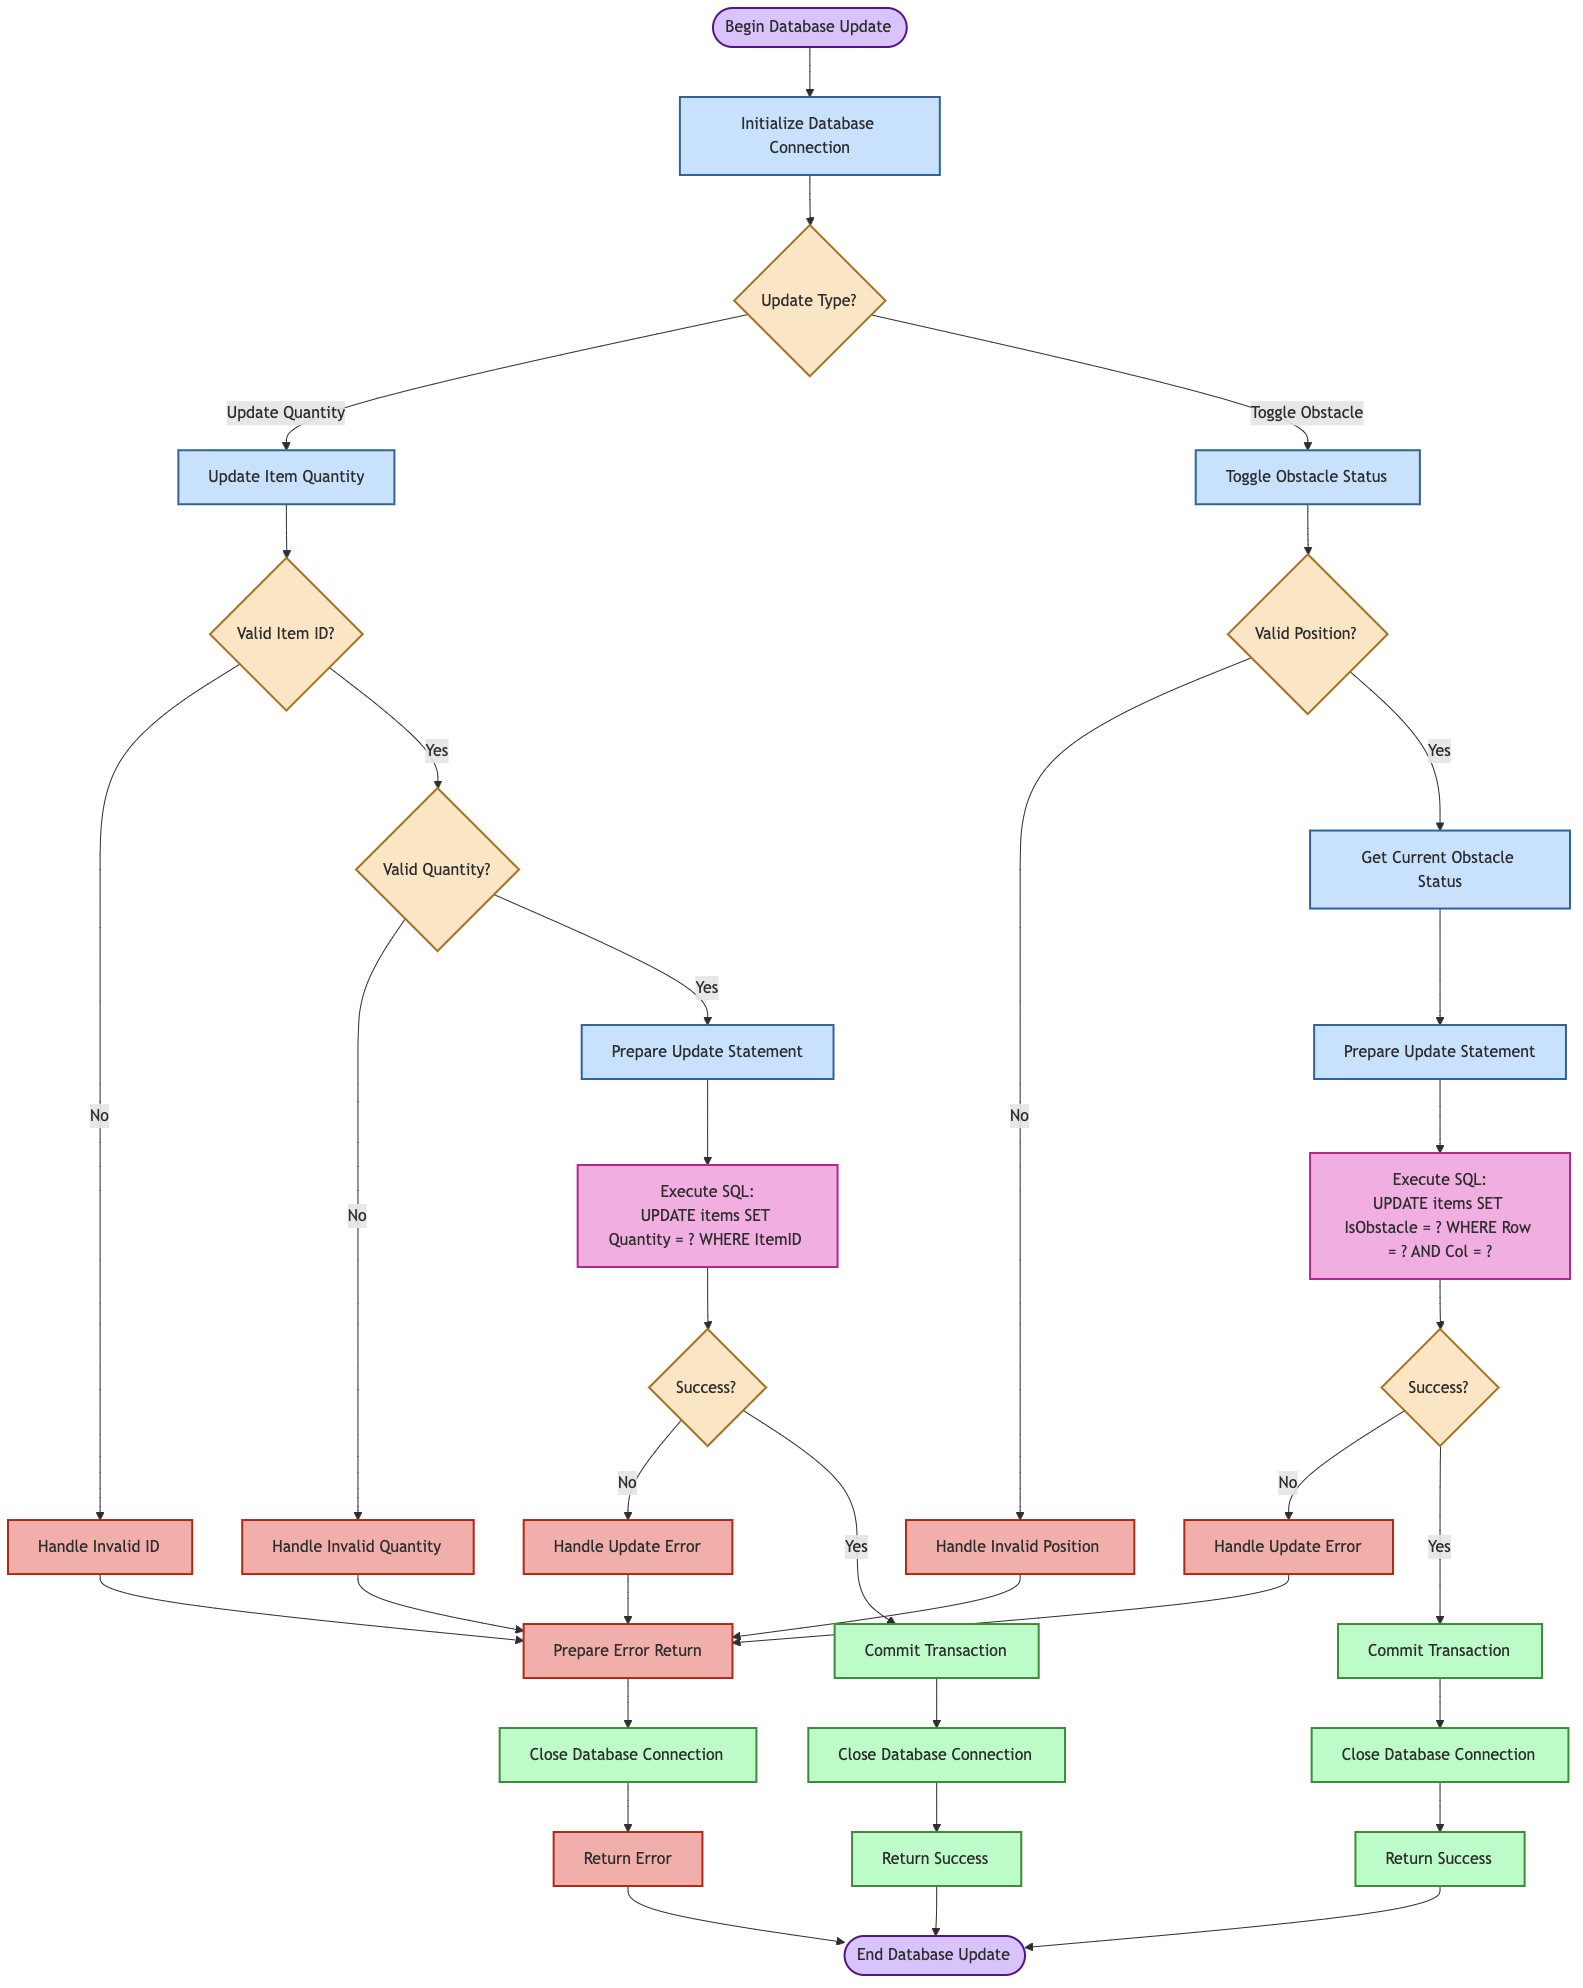
\includegraphics[width=0.9\linewidth]{Flowcharts/dbwrite.png}
\end{figure}

\newpage

\subsection{Configuration}

\begin{figure}[htbp]
    \centering
    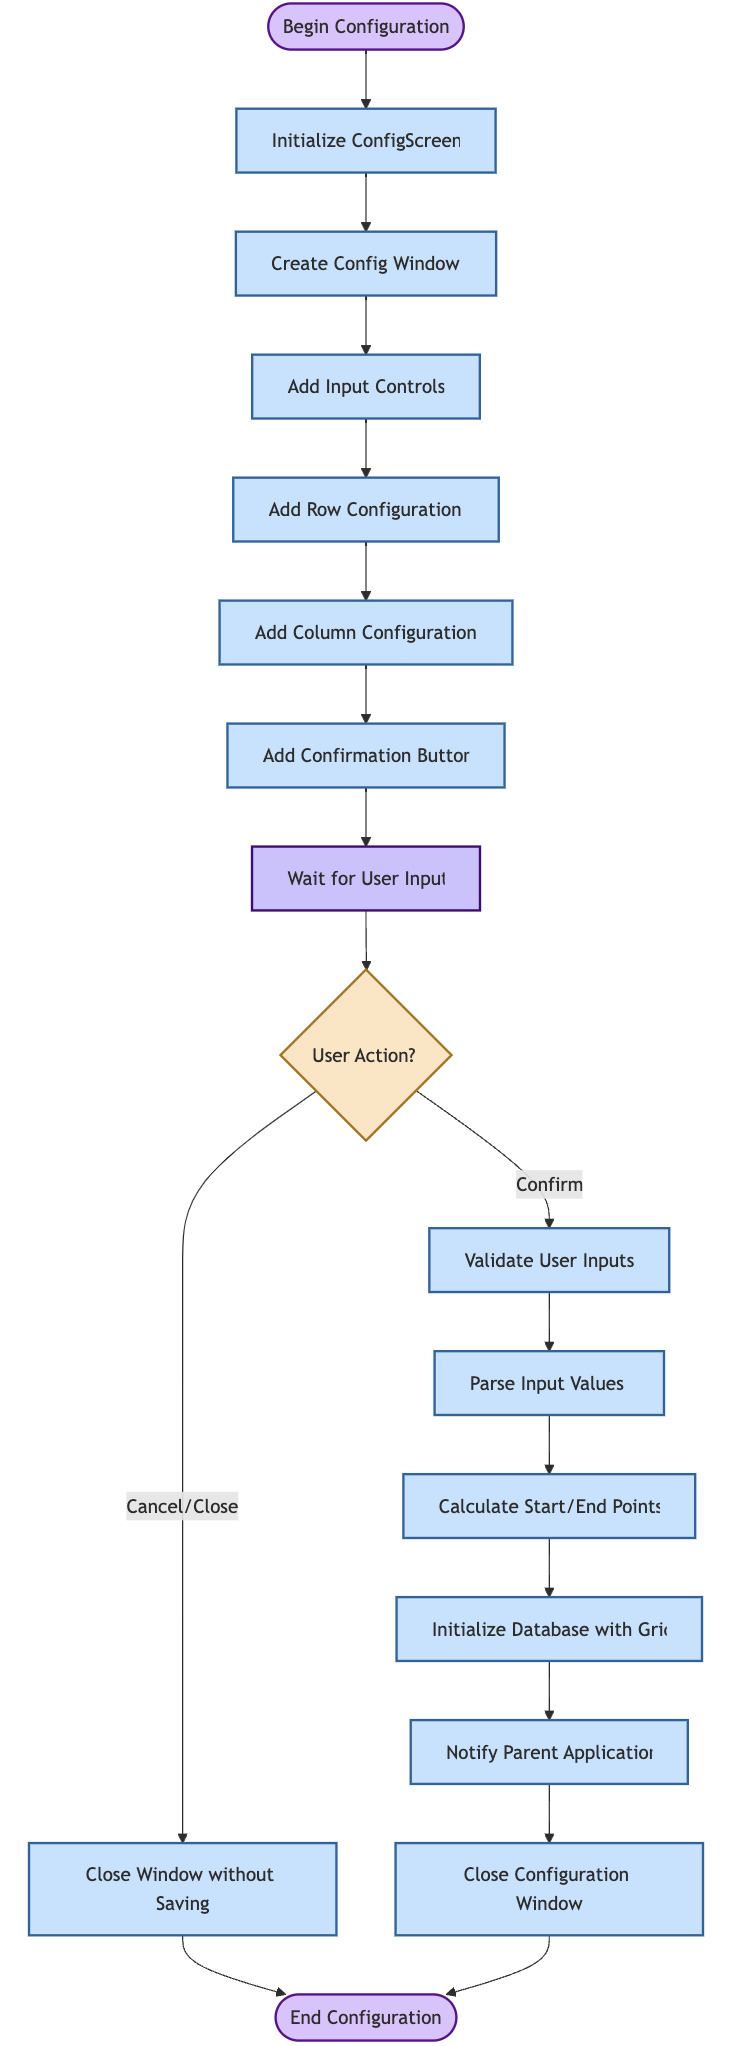
\includegraphics[width=0.4\linewidth]{Flowcharts/config1.png}

\end{figure}

\newpage

\subsection{JSON import/export}

\begin{figure}[htbp]
    \centering
    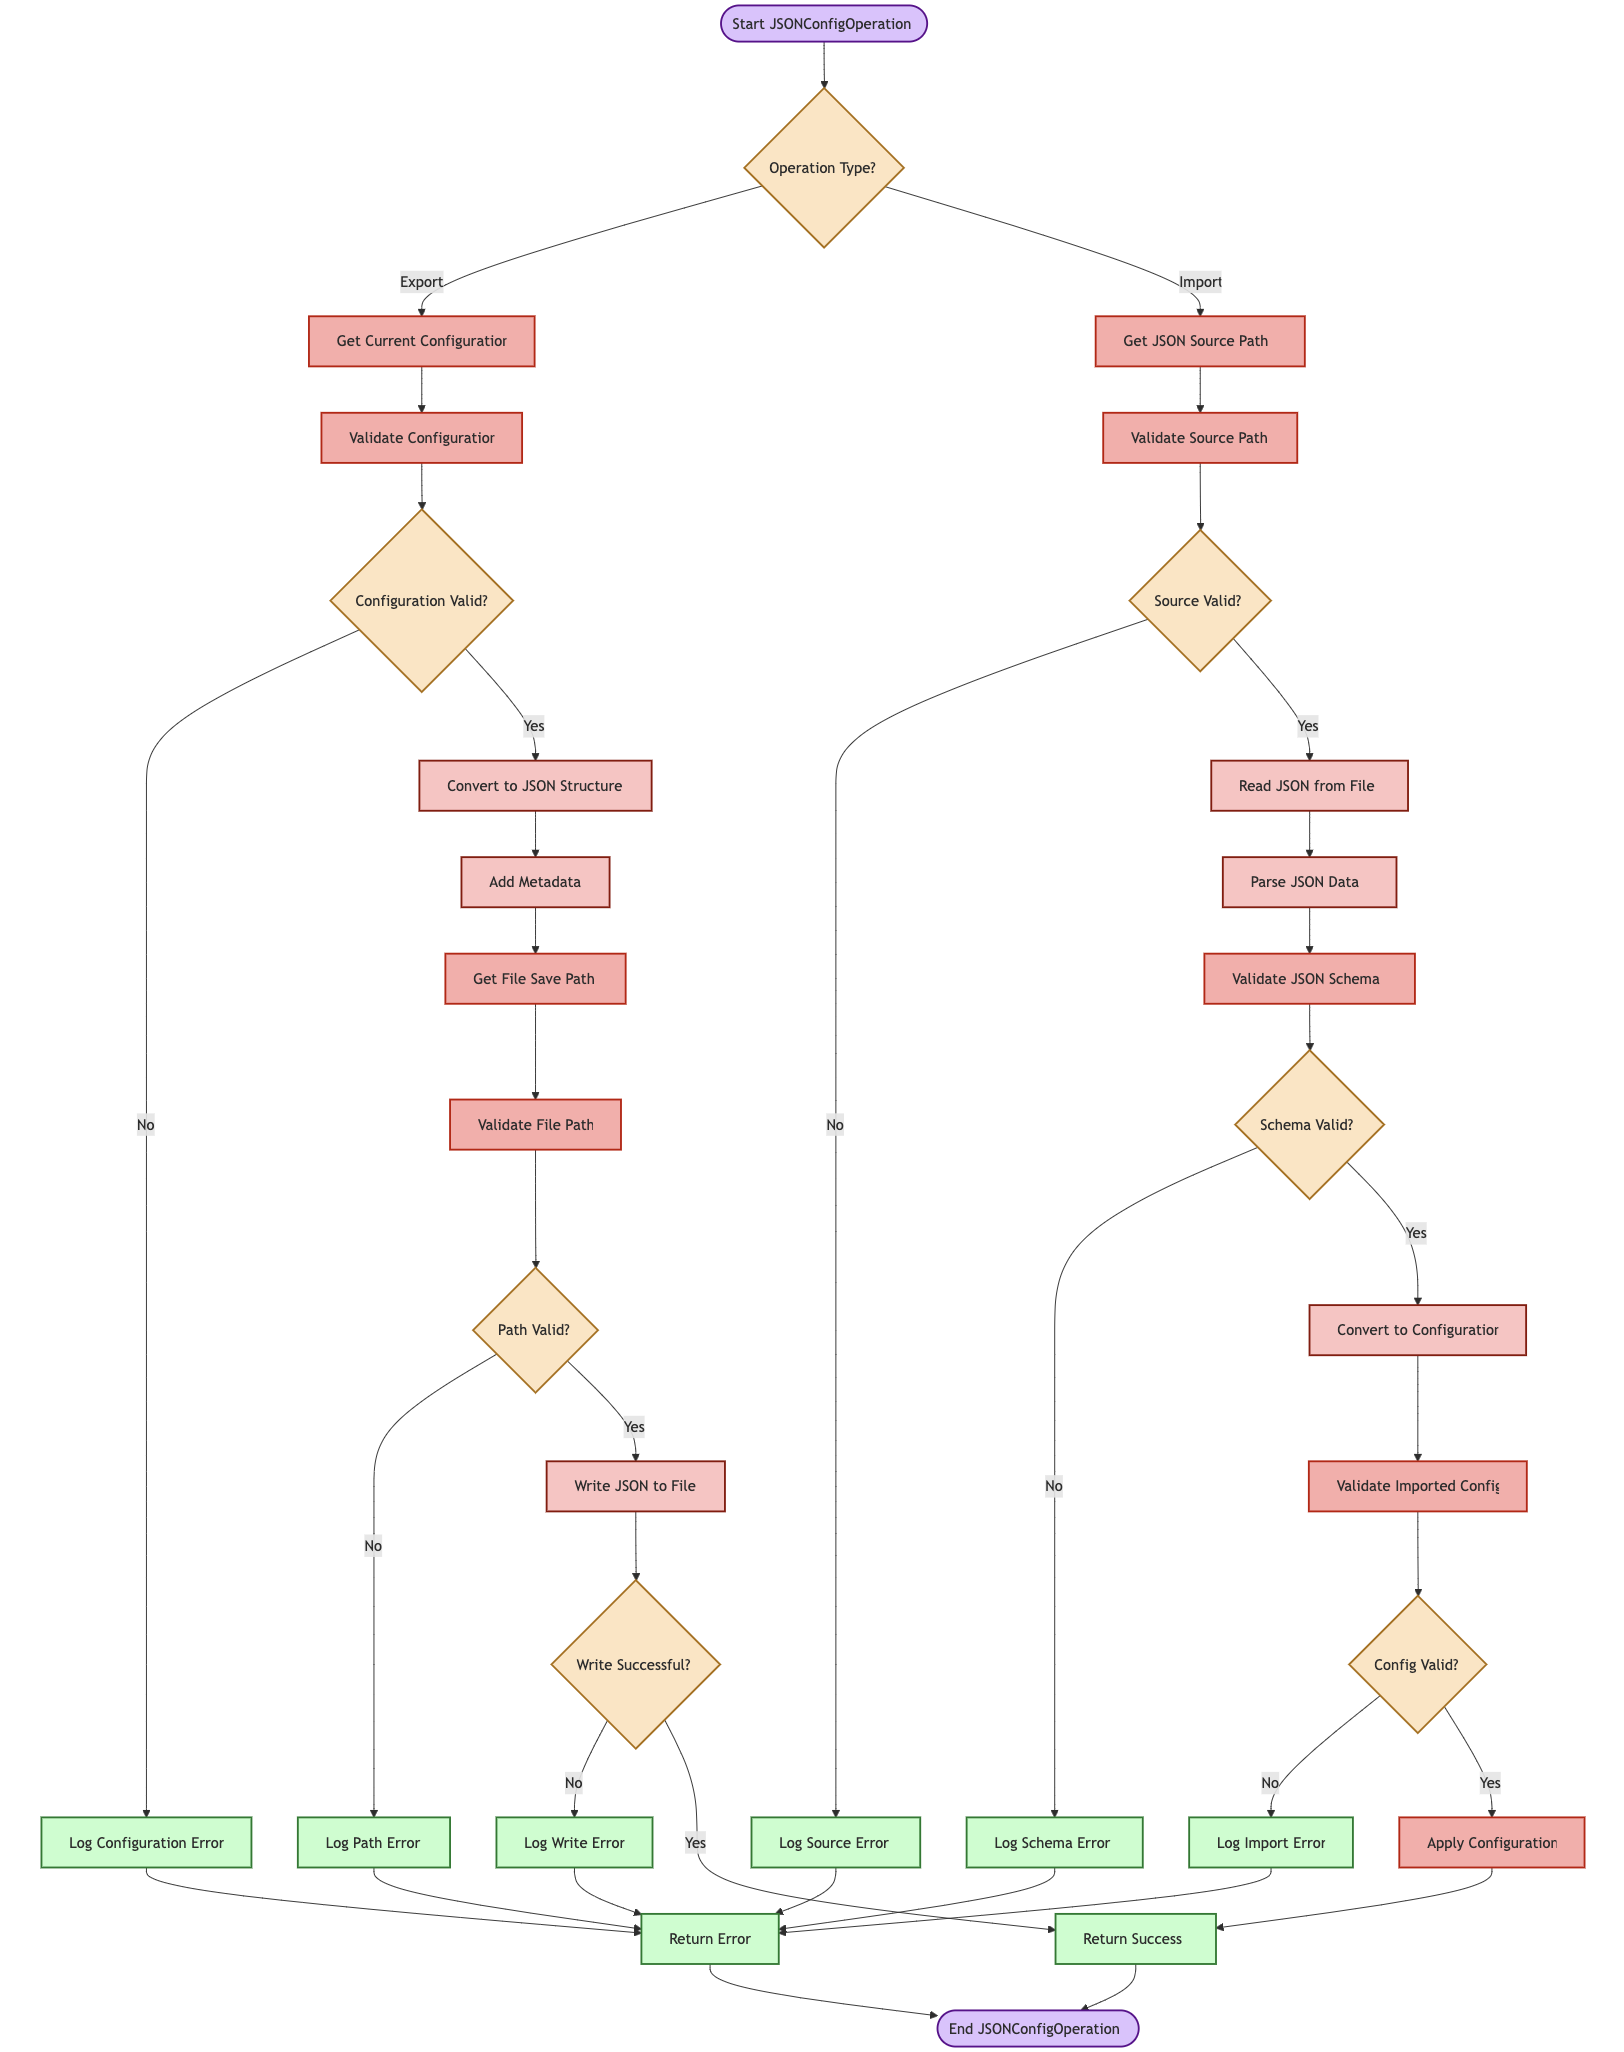
\includegraphics[width=0.8\linewidth]{Flowcharts/json.png}

\end{figure}

\newpage

\subsection{Possible refinements}

\begin{figure}[!htbp]
	\centering
	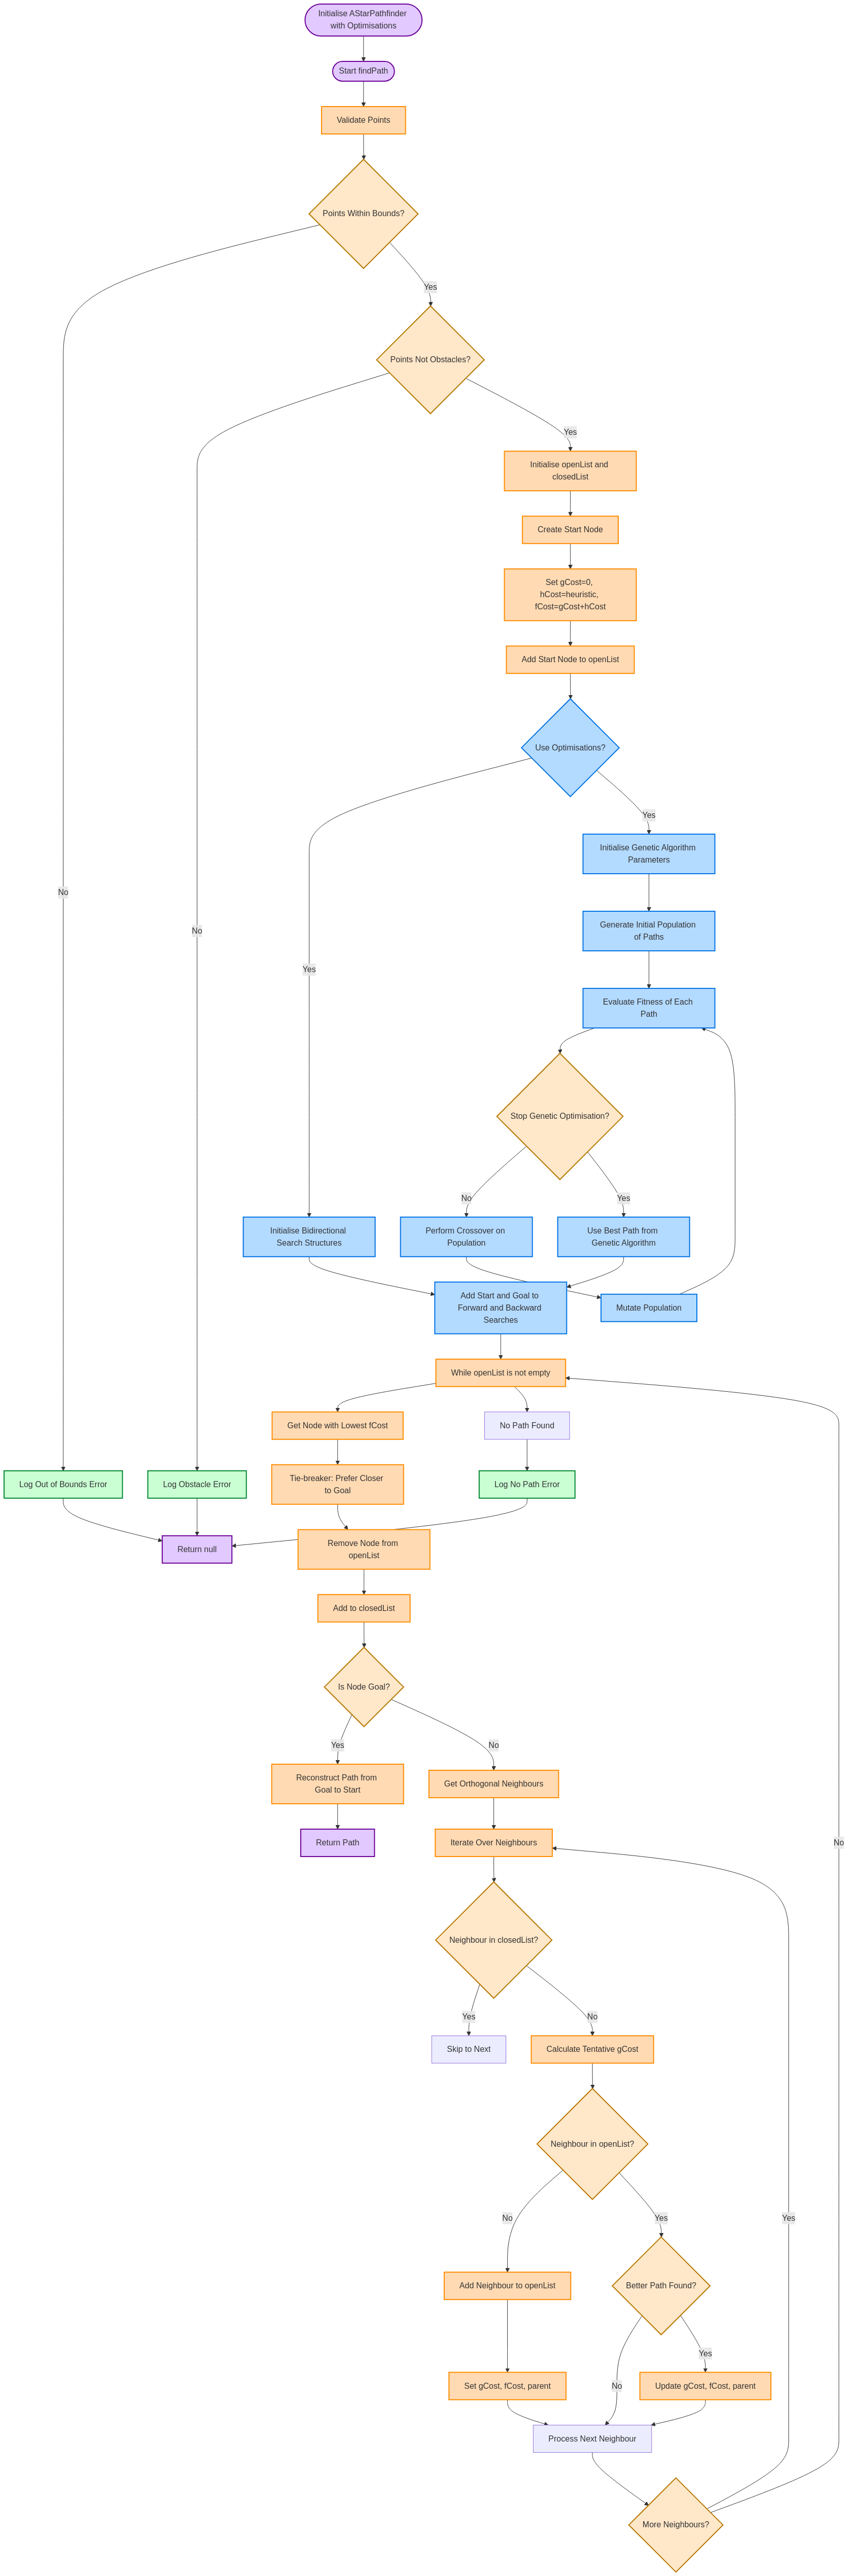
\includegraphics[width=0.4\linewidth]{Flowcharts/optimisedastar.png}
\end{figure}

\newpage
\section{Usability}

On the subject of GUIs, what rules should a GUI actually follow to be optimal for the end user? The guidelines below are a subset of the ones that form the guides of both the Google and the Adobe design team, and hence appropriate due to both their success and accessibility. \textsuperscript{\cite{design1, design2}}

\subsection{Guidelines}
\begin{itemize}
\item \textbf{Visibility of system status:} Users should always be informed of system operations with easy to understand and highly visible status displayed on the screen within a reasonable amount of time.

\item \textbf{Consistency and standards:} Interface designers should ensure that both the graphic elements and terminology are maintained across similar platforms. For example, an icon that represents one category or concept should not represent a different concept when used on a different screen.

\item \textbf{Error prevention:} Whenever possible, design systems so that potential errors are kept to a minimum. Users do not like being called upon to detect and remedy problems, which may on occasion be beyond their level of expertise. Eliminating or flagging actions that may result in errors are two possible means of achieving error prevention.

\item \textbf{Recognition rather than recall:} Minimise cognitive load by maintaining task-relevant information within the display while users explore the interface. Human attention is limited and we are only capable of maintaining around five items in our short-term memory at one time. Due to the limitations of short-term memory, designers should ensure users can simply employ recognition instead of recalling information across parts of the dialogue. Recognising something is always easier than recall because recognition involves perceiving cues that help us reach into our vast memory and allowing relevant information to surface. For example, we often find the format of multiple choice questions easier than short answer questions on a test because it only requires us to recognise the answer rather than recall it from our memory.

\item \textbf{Aesthetic and minimalist design:} Keep clutter to a minimum. All unnecessary information competes for the user's limited attentional resources, which could inhibit user's memory retrieval of relevant information. Therefore, the display must be reduced to only the necessary components for the current tasks, whilst providing clearly visible and unambiguous means of navigating to other content.

\end{itemize}

\newpage

\subsection{Configuration Screen Analysis}
\begin{figure}[!htbp]
    \centering
    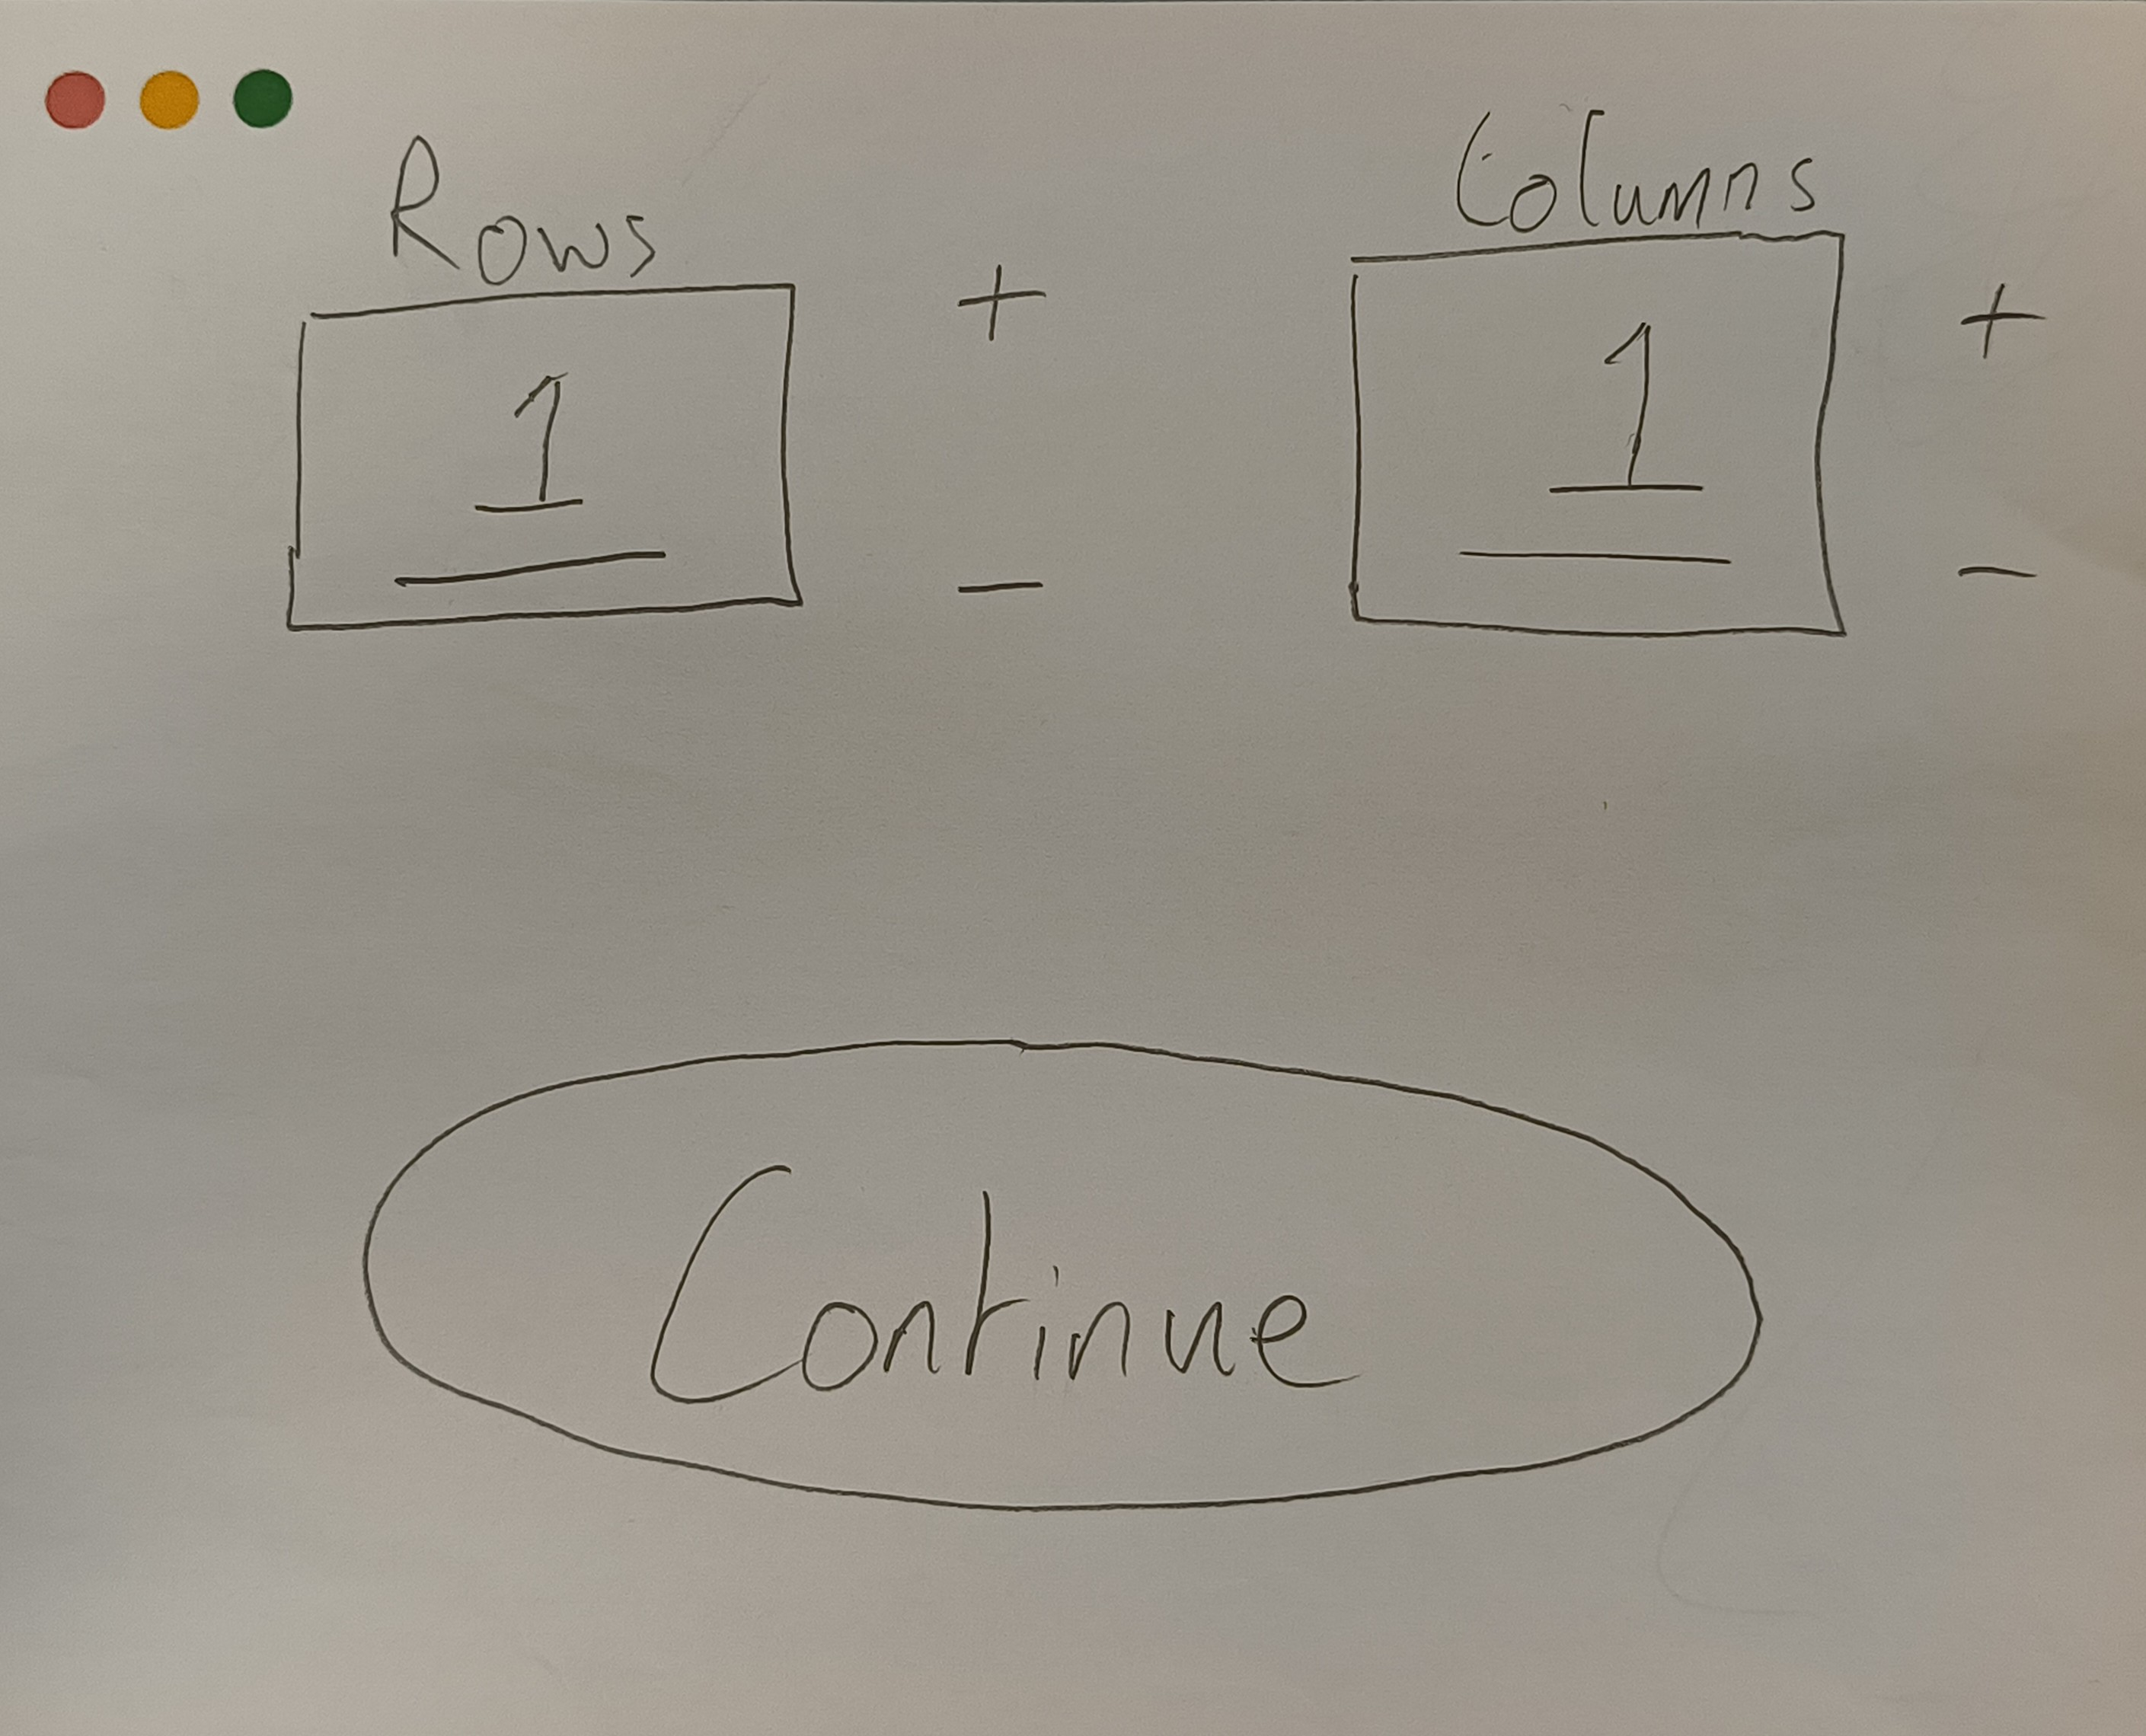
\includegraphics[width=1\linewidth]{Images/InitGUI.jpg}
    \caption{- A hypothetical configuration window prior to running the main program.}
\end{figure}

\newpage



\subsubsection{Guideline alignment:}


    \begin{itemize}
        \item Visibility of System Status
        \begin{itemize}
            \item Clear numeric displays for rows/columns
            \item Plus/minus controls provide immediate feedback
            \item "Continue" button shows clear next step
    
        \end{itemize}
    \end{itemize}
    
    \begin{itemize}
        \item Error Prevention
        \begin{itemize}
            \item Bounded input fields prevent invalid grid sizes
            \item Plus/minus buttons prevent text input errors
            \item Single "Continue" path reduces navigation errors
        \end{itemize}
    \end{itemize}
    
    \begin{itemize}
        \item Recognition vs Recall
    
        \begin{itemize}
            \item Labelled "Rows" and "Columns" fields
            \item Simple numeric input reduces cognitive load
            \item Clear action button labelled "Continue"
        \end{itemize}
    \end{itemize}
    
    
    \begin{itemize}
        \item Aesthetic/Minimalist
    
        \begin{itemize}
            \item Only essential grid setup controls
            \item Clean layout without distracting elements
            \item Logical grouping of related controls
        \end{itemize}
\end{itemize}



\begin{itemize}
    \item Consistency

    \begin{itemize}
        \item Uniform input field styling
        \item Consistent plus/minus button placement
        \item Standard window controls
    \end{itemize}
\end{itemize}


\subsubsection{Usability Analysis:}

The numeric input fields with increment/decrement controls are an optimal solution for grid dimension entry, as there are many variants of warehouse that can be constructed via row and column definition - this allows for faster input of the desired warehouse dimensions. \newline The interface's spatial organisation leverages natural reading patterns and mental models by arranging elements in a logical left-to-right, top-to-bottom flow that correlates with the final grid structure. \newline The centrally positioned continue button serves as a clear visual endpoint, while the minimalist two-field design effectively mitigates a cluttered and hard-to-navigate interface that would otherwise arise if this and the main program was incorporated as one window.

\newpage

\subsection{Main Screen Analysis}

\begin{figure}[!htbp]
    \centering
    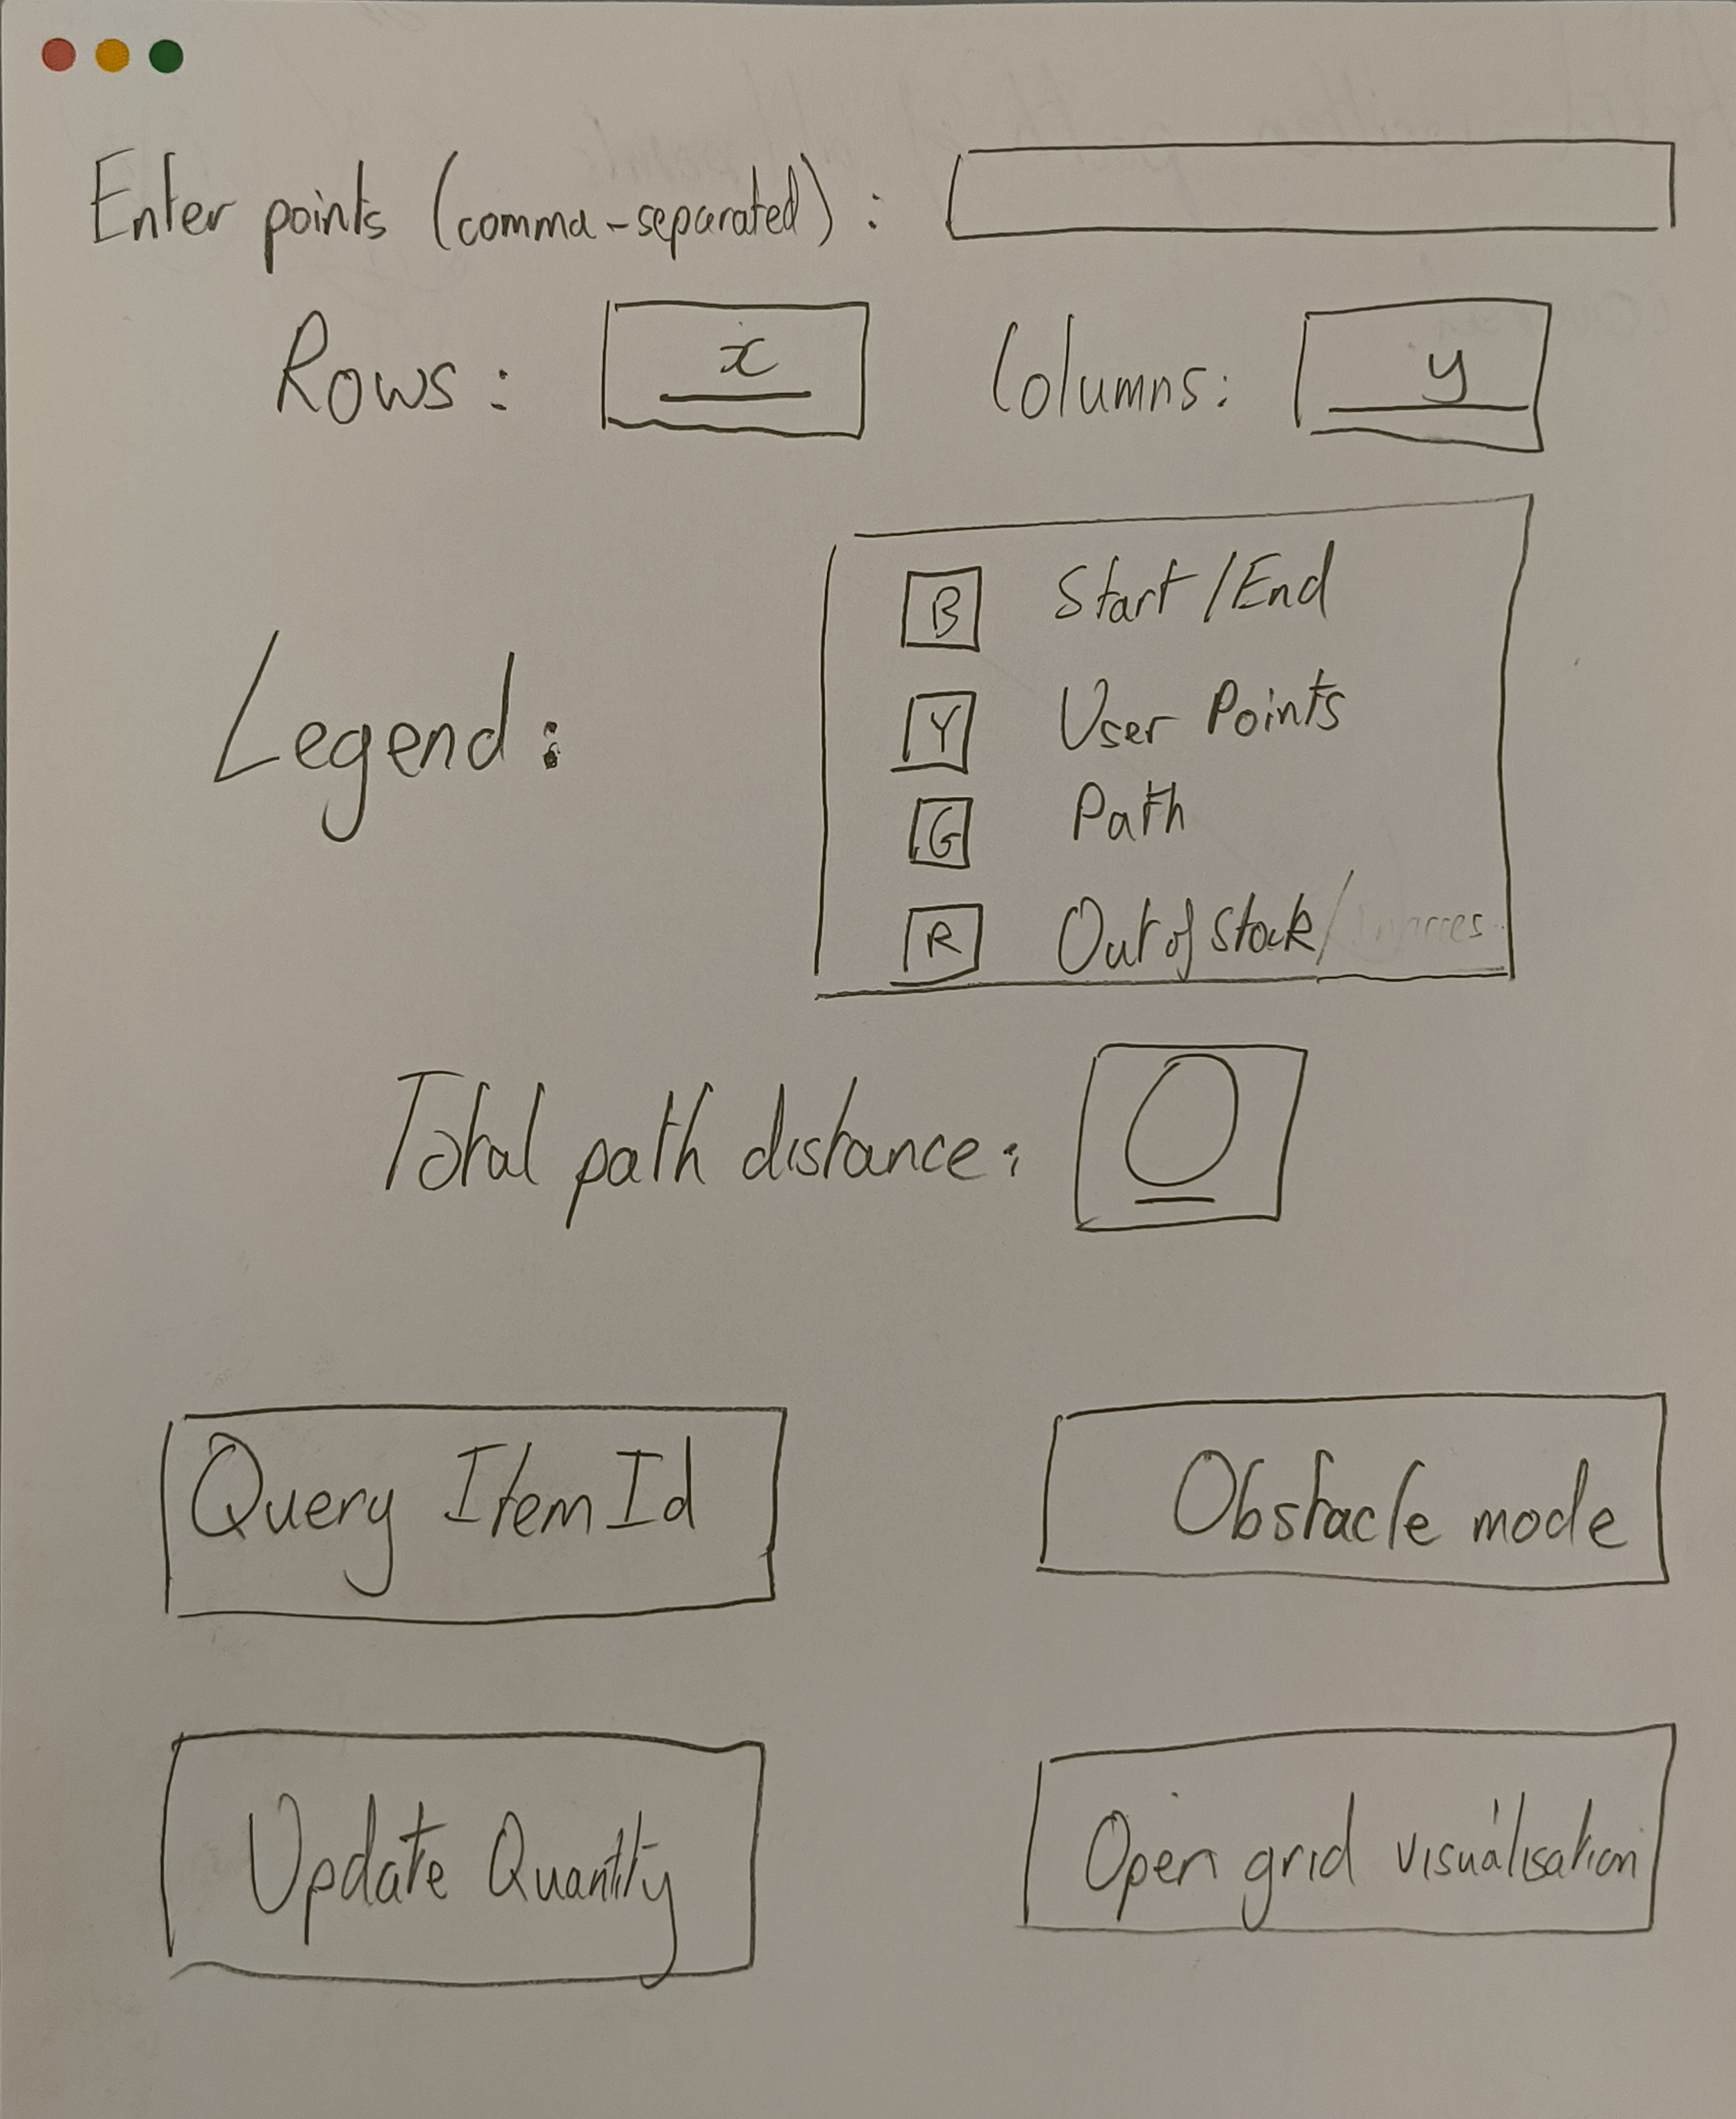
\includegraphics[width=1\linewidth]{Images/GUI.jpg}
    \caption{- The main window of StockBot}
\end{figure}

\newpage




\subsubsection{Guideline alignment:}

    \begin{itemize}
        \item Visibility of System Status
        \begin{itemize}
            \item Legend shows current grid state meanings
            \item Total path distance display
            \item Clear input field for points
    
        \end{itemize}
    \end{itemize}
    
    \begin{itemize}
        \item Error Prevention
        \begin{itemize}
            \item Explicit format guidance ("comma-separated")
            \item Legend prevents colour interpretation errors
            \item Clear button labels prevent navigation mistakes
        \end{itemize}
    \end{itemize}
    
    \begin{itemize}
        \item Recognition vs Recall
    
        \begin{itemize}
            \item Complete legend eliminates colour code memorisation
            \item Input format shown directly above field
            \item Descriptive button labels
        \end{itemize}
    \end{itemize}
    
    
    \begin{itemize}
        \item Aesthetic/Minimalist
    
        \begin{itemize}
            \item Logical grouping of controls
            \item Clean separation of input/visualisation areas
            \item Essential information only
        \end{itemize}
\end{itemize}

This interface is consistent for the same reasons as the configuration screen.

\subsubsection{Usability Analysis}
The implementation of a text entry field for input is superior as it offers flexibility and choice to the user, while remaining as simple as possible. While I did consider multiple drop-down menus, one for the number of points and the others for items, I dismissed the idea on the fact that a large warehouse would lead to a very cluttered UI. This design choice also allows for easier parsing, as the entire entry can be taken at once rather than extraction from each drop-down menu. \newline The interface architecture establishes clear visual hierarchies that guide users through complex tasks while maintaining accessibility to all functions. The prominent placement of primary operations (point entry and grid visualisation) balanced against the discrete positioning of secondary functions (querying, updating) creates an intuitive interaction flow. \newline
While I initially did not want to include a legend, adding one would benefit the user; it eliminates cognitive overhead associated with colour mapping recall.

\newpage

\subsection{Grid Visualisation}

\begin{figure}[!htbp]
    \centering
    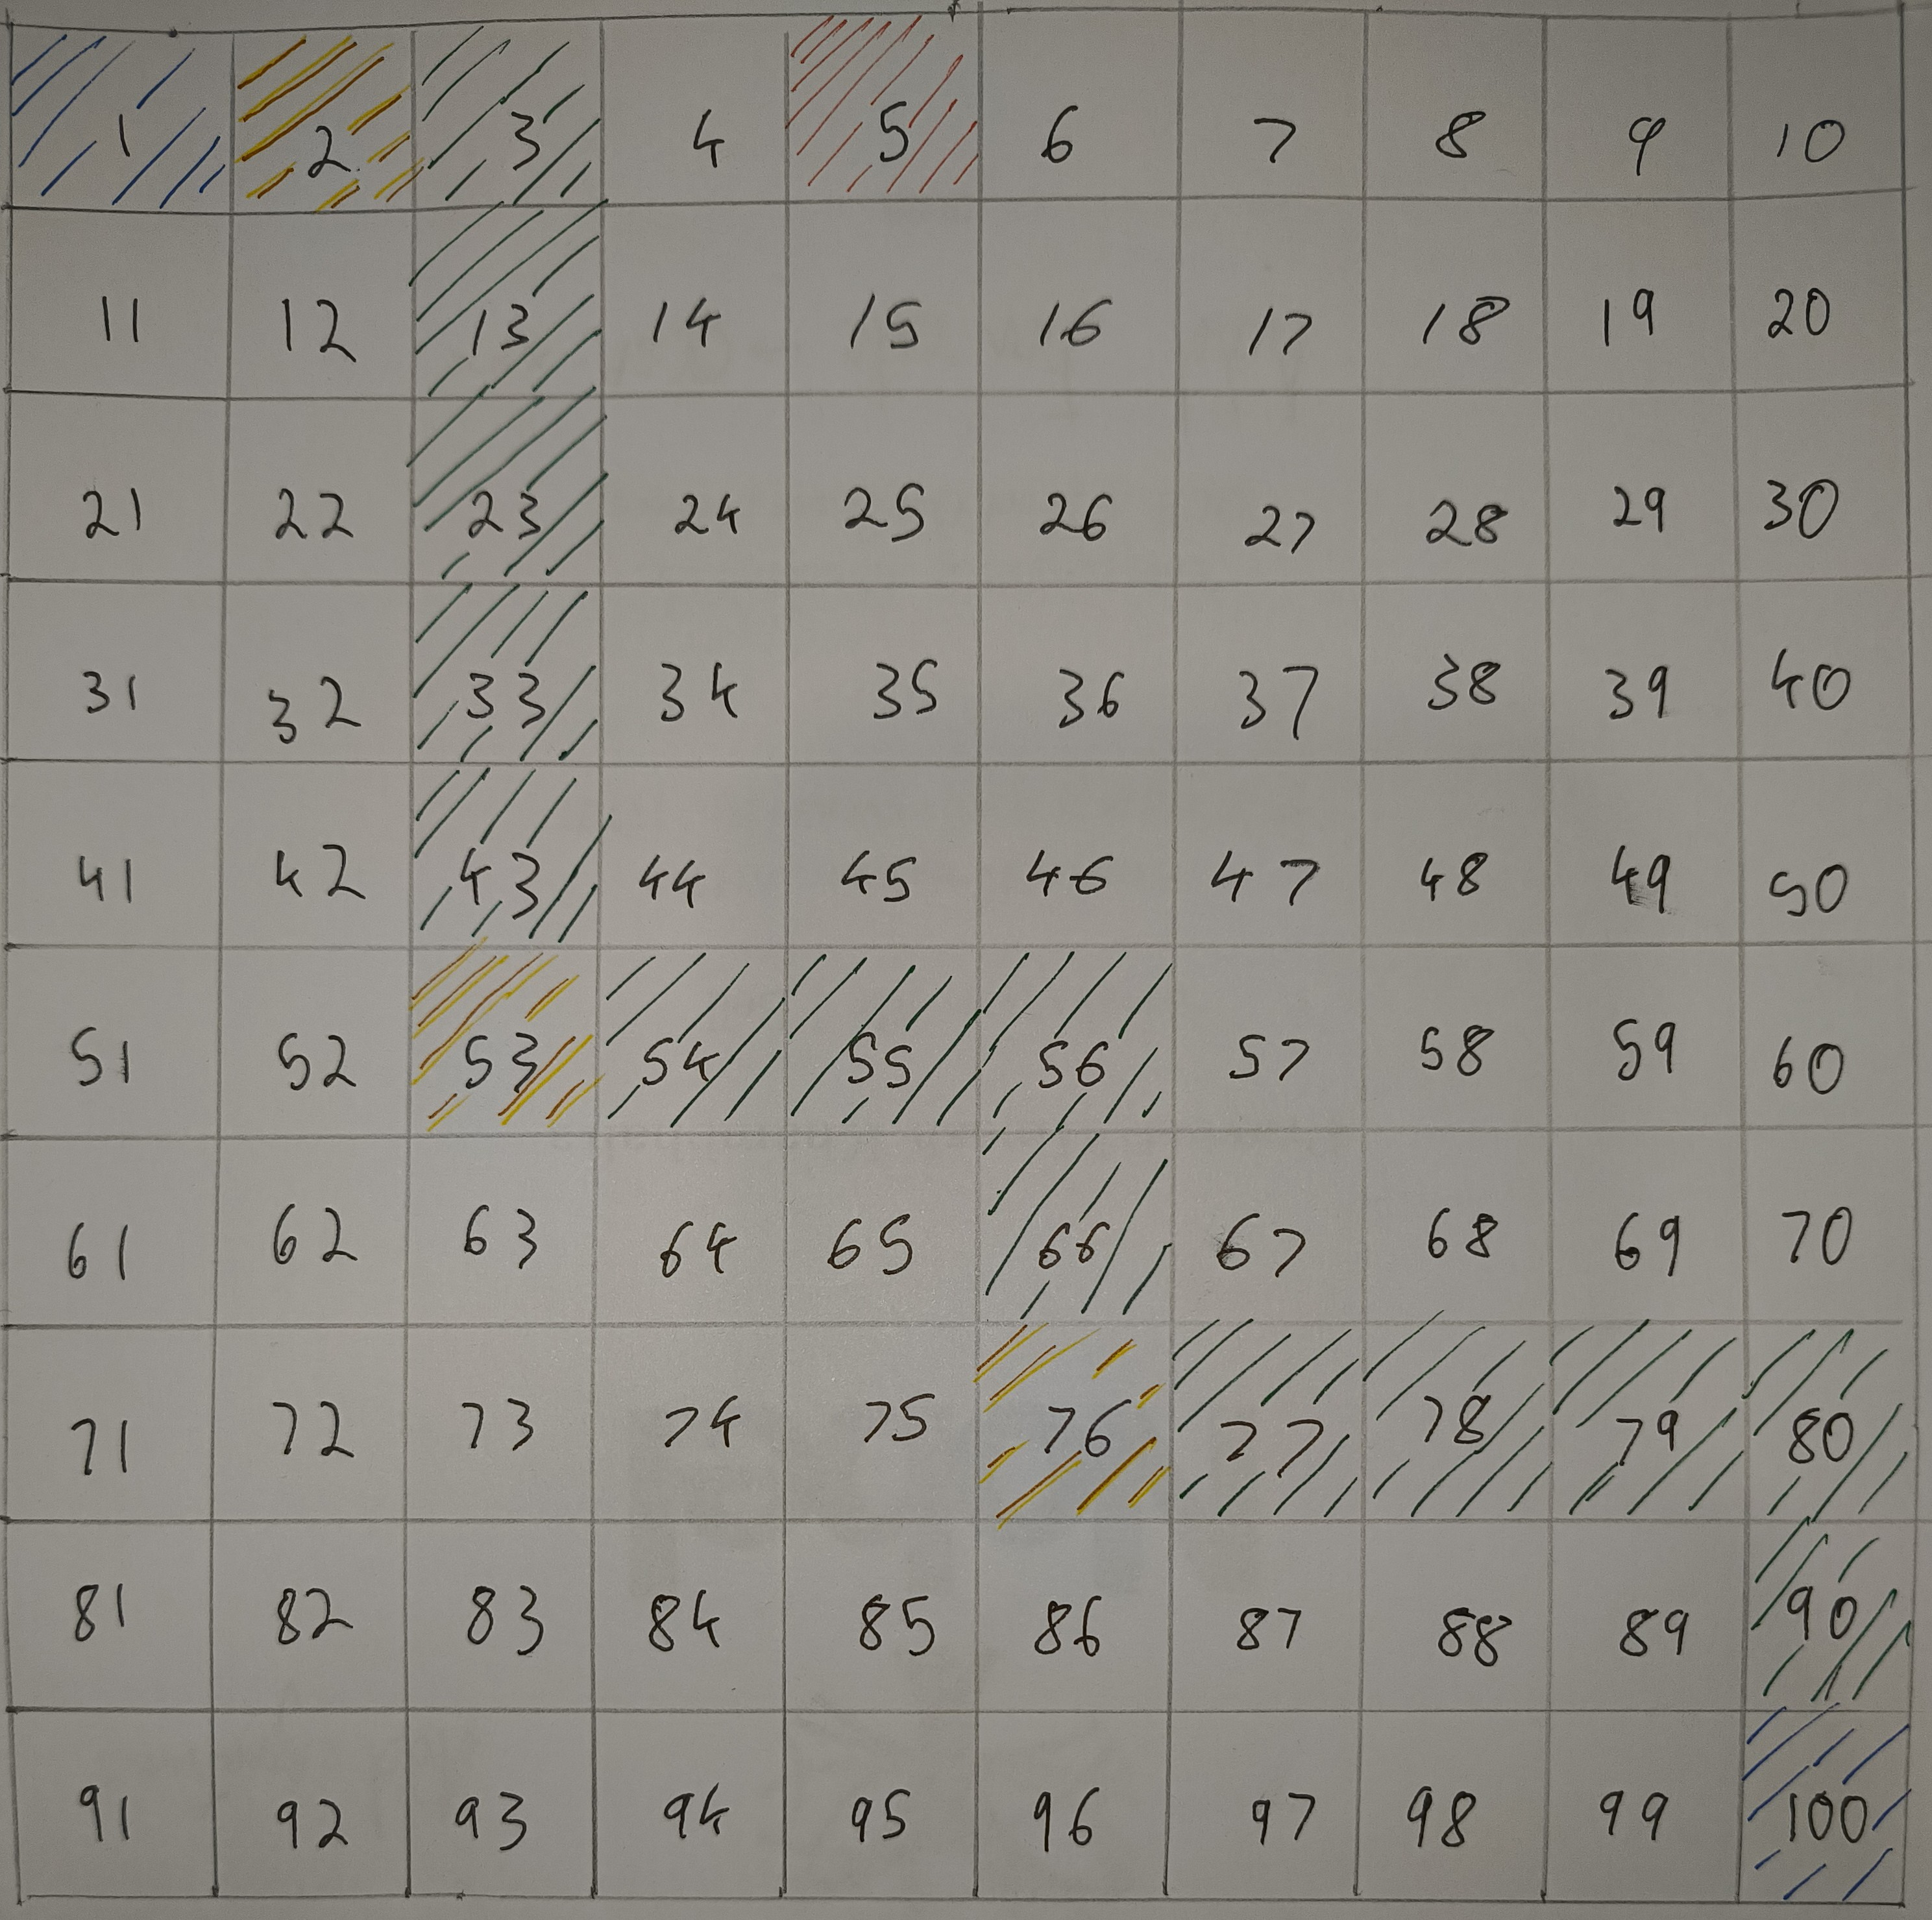
\includegraphics[width=1\linewidth]{gridvisual.jpg}
    \caption{- The visualisation of the path.}
\end{figure}

\newpage

\section{Unifying the algorithms}

While the algorithms are complete, the solution has not yet been unified into a functional app; as I have used OOP principles in the code, it will be much easier to create a working prototype. See section x.x.x for the benefits OOP provides. The goal is to combine the shortest path algorithms (SPA), the graphical user interface (GUI), and the database management system into a cohesive application structured around these three core features. I have broken down the unification process into the module breakdown, the role of each module, the key functions and the interactions between modules.

\subsection{Key modules breakdown}

\subsubsection{GUI}
    
This serves as the main entry point for the program. It will manage user input, visualisation, and overall coordination of the application. When necessary, the program will call methods or functions from the SPA and Database modules for computation and data management respectively.

\begin{itemize}
    \item Primary Role: Acts as the main control system and interface between the user and the computational/backend modules.
    \item Key Functions:
        \begin{itemize}
            \item Input Collection: Accepts user inputs like setting obstacles, defining waypoints, and initiating pathfinding.
            \item Visualisation: Displays the grid and highlights paths, obstacles, and waypoints for the user.
            \item Interaction with SPA: Passes grid configurations and waypoints to the SPA module to compute the shortest path.
            \item Interaction with Database: Calls Database to save or load grid states, configurations, or paths.
        \end{itemize}
    \item Effect of unification: \newline
    The GUI acts as a bridge between the user and the underlying logic. It passes the data it collects (like grid configurations or waypoints) to SPA for computations and calls Database for storage tasks. All modules are coordinated through the GUI, making it the central orchestrator.
\end{itemize}


\subsubsection{SPA}
This contains the core algorithms for computing the shortest path. It contains logic for handling grid data, waypoints and pathfinding. In the program, it will act as a processing unit, receiving data from the GUI, performing computations, and returning results.

\begin{itemize}
    \item Primary Role: Implements and executes the algorithms that compute the shortest path on a grid.
    \item Key Functions:
        \begin{itemize}
            \item Algorithm Logic: Encapsulates shortest path algorithms.
            \item Data Handling: Accepts grid configuration and waypoints from GUI and processes them to compute the desired path.
            \item Result Output: Returns the computed path to the GUI for visualisation.
        \end{itemize}
    \item Effect of unification: \newline
        SPA is isolated from the GUI and database logic, focusing purely on computation. It accepts data from GUI and processes it using the appropriate algorithm. By keeping the logic separate, the module remains reusable and scalable, allowing future algorithms to be added without modifying the GUI or database.
\end{itemize}



\subsubsection{Database}
This will provides data persistence by saving and loading grid configurations, waypoints, and paths. It will ensures the program can maintain state across sessions, enabling users to resume from where they left off.

\begin{itemize}
    \item Primary Role: Stock management - ensuring stock is present and if not, to skip over the item.
    \item Key Functions:
        \begin{itemize}
            \item Data Integrity: Ensures that saved data remains consistent and valid.
            \item Stock assignment: Allows for items to be assigned to positions in the warehouse
            \item Stock verification: Verifies that stock exists and if not, to remove the item from queue.
        \end{itemize}
    \item Effect of unification: \newline
        Database connects with GUI to store or retrieve data as requested by the user. This separation of concerns allows the GUI to focus on interaction and visualization, while the database handles storage operations independently.
\end{itemize}

These are just the key features that are integral to my solution. I have also included some quality-of-life features that I feel the stakeholders would benefit from, which I will include if time permits.

\newpage

\subsection{A unified implementation}

\begin{figure}[htbp!]
    \centering
    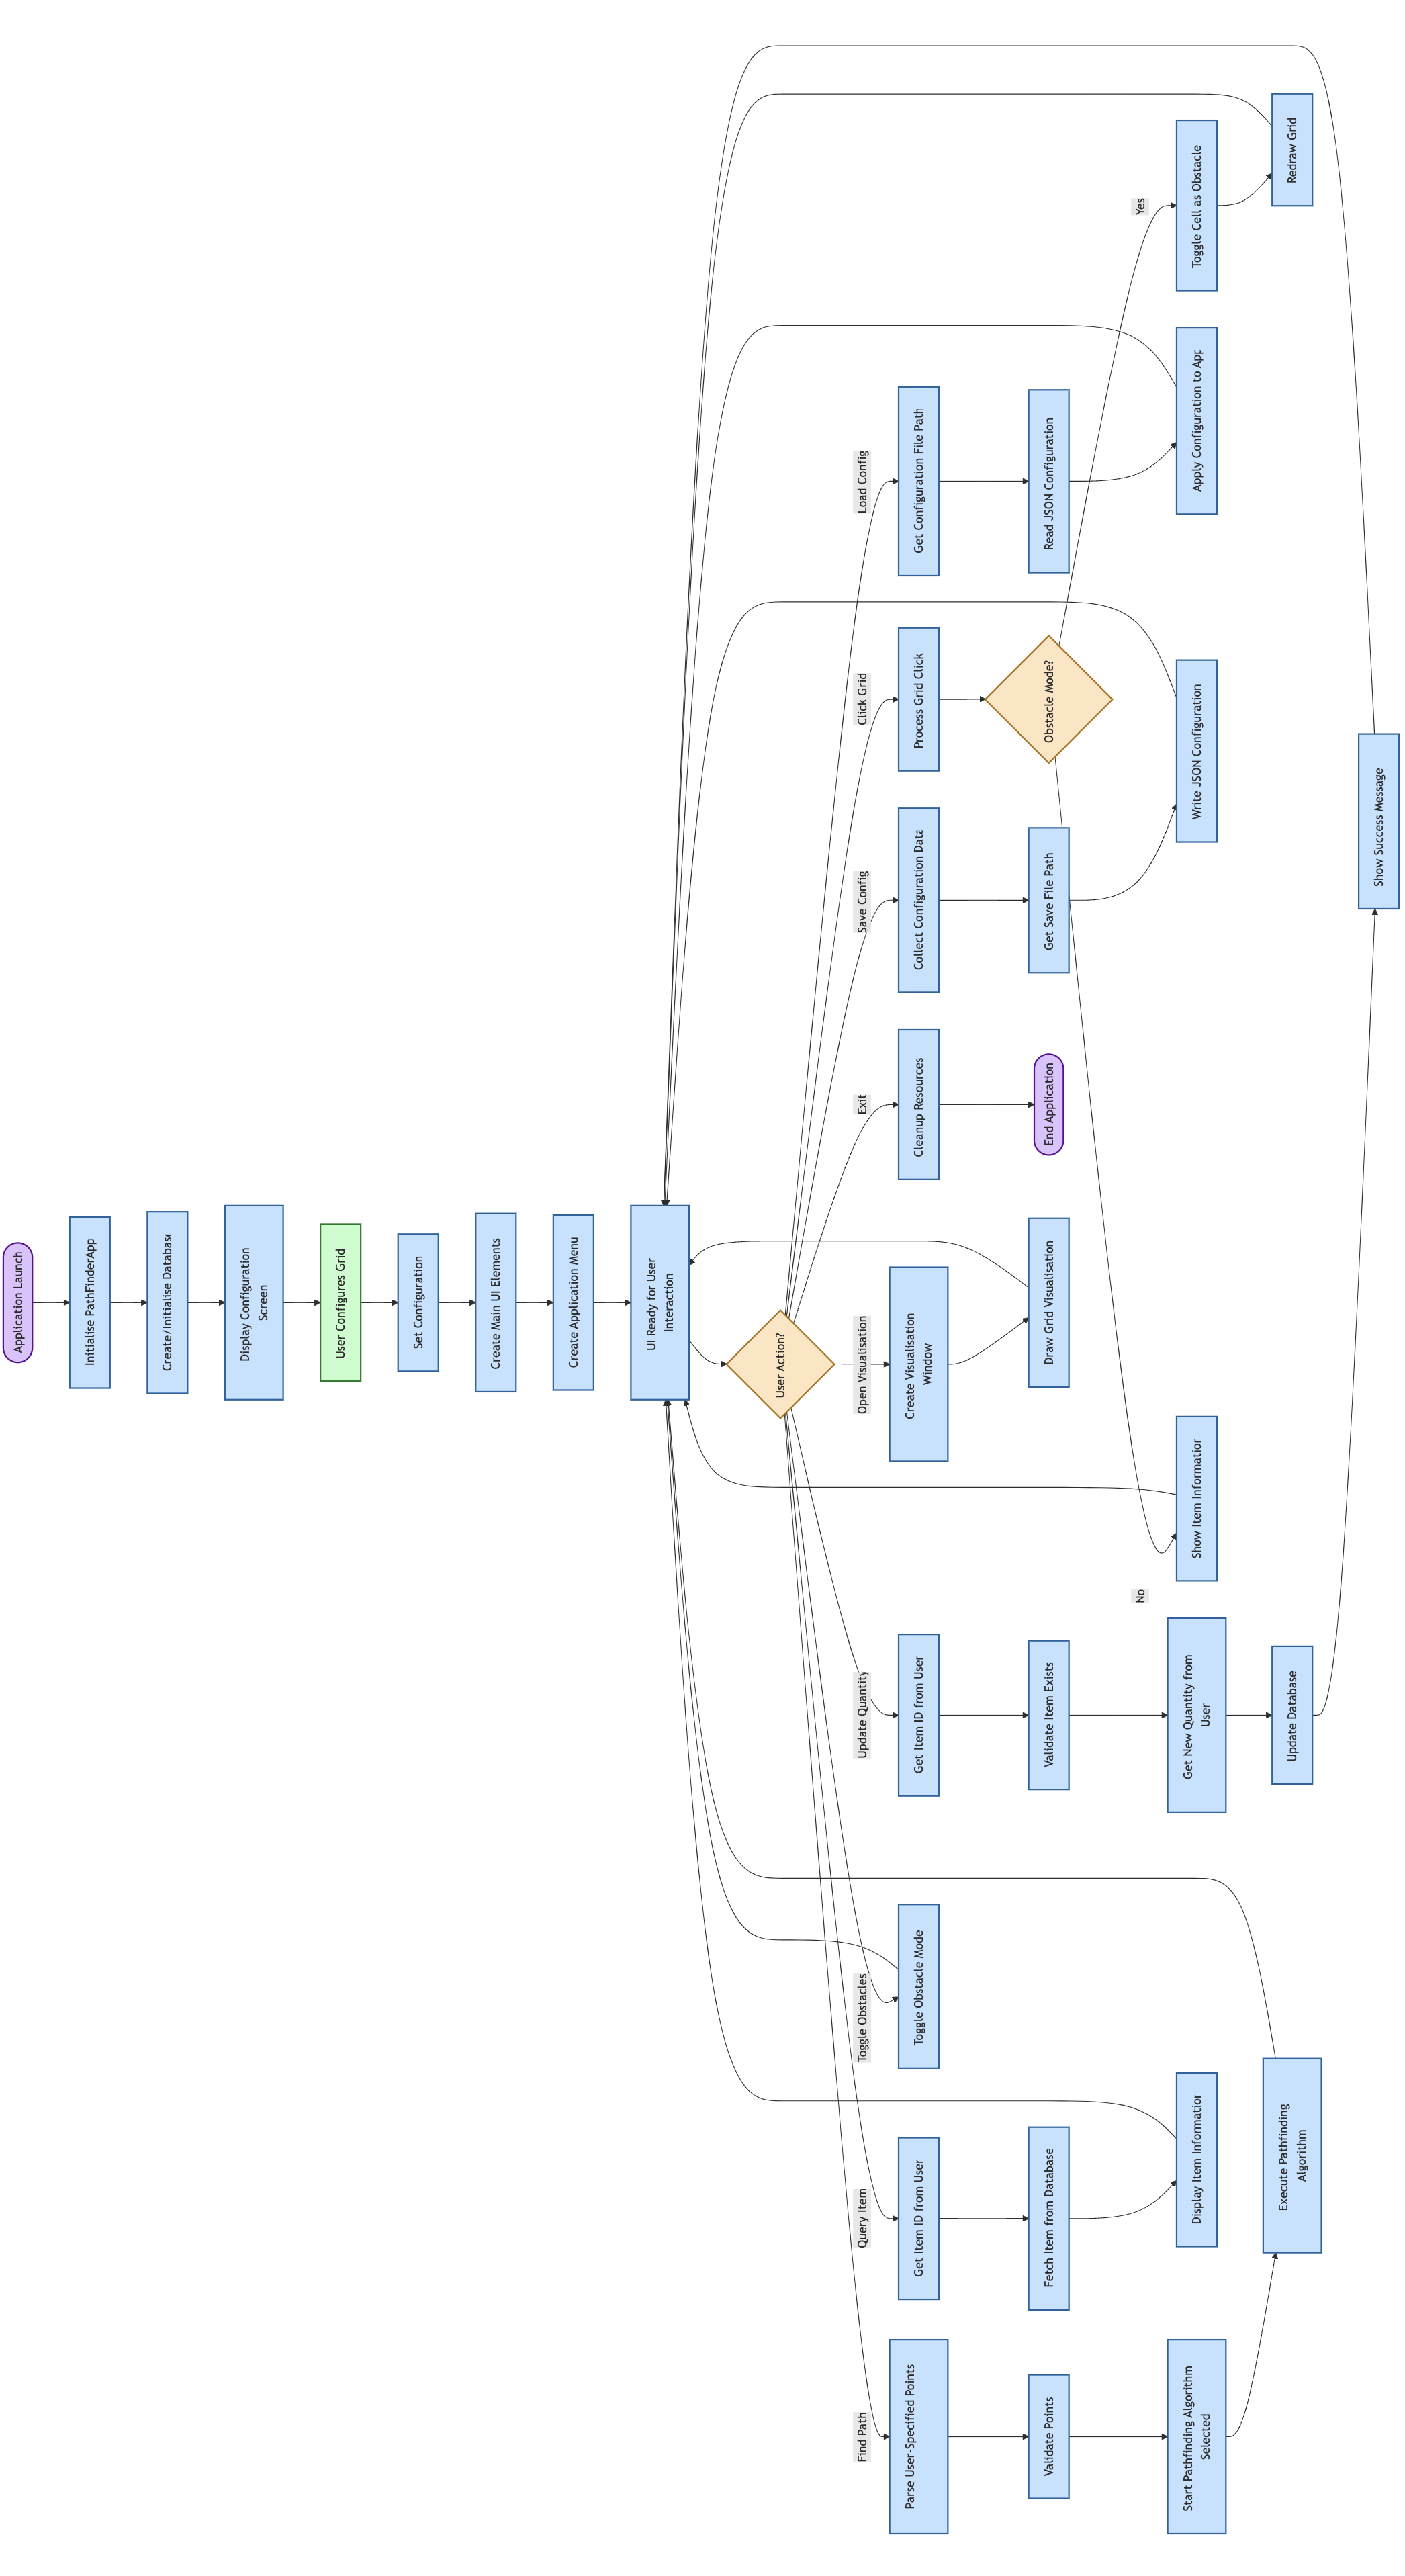
\includegraphics[width=0.7\linewidth]{Flowcharts/Unified.png}

\end{figure}

\newpage

\section{Test data}

\subsection{Standard data}

I will be using the following data as a boilerplate environment for post-development in addition to the test data below. These are the parameters I will set for generic testing for the stakeholders. They will test it as they see fit and report back with any final feedback. I will not be providing them with exact data as I wish to simulate a real environment and hence test this software in a less controlled manner; this is why this data is more ambiguous.

\begin{itemize}
	\item Grid layout: 15 x 15 default, user discretion to change
	\item Random database generation
	\item Point selection varying between 2 and 224, using a random number generator
	\item Number of points varying between 1 and 25, using a random number generator
\end{itemize}

\subsection{During development}

These tests will be performed during development. The test IDs are in the format TA.B.C where A is the sprint number, B is the iteration number and C is the test number. T.x.F tests are the pre-determined tests that will be performed by stakeholders, while T.x.x tests will be used to test each iteration.

\begin{table}[htbp]
	\centering
	\begin{tabularx}{\textwidth}{|l|X|}
		\hline
		\textbf{ID} & \textbf{Description} \\
		\hline
		T1.F.1 & Path found using input points \\
		\hline
		T1.F.2 & Input invalid points (letters, numbers and symbols) \\
		\hline
		T1.F.3 & Input no points \\
		\hline
	\end{tabularx}
	\caption{Pre-determined tests}
\end{table}

\begin{table}[htbp]
	\centering
	\begin{tabularx}{\textwidth}{|l|X|}
		\hline
		\textbf{ID} & \textbf{Description} \\
		\hline
		T1.1.1 & Input 0,0 and 9,9 \\
		\hline
		T1.1.2 & Input 1,2 and 5,7 \\
		\hline
		T1.1.3 & Input -1,-1 and 4,8 \\
		\hline
		T1.1.4 & Input 0,1 and 10,10 \\
		\hline
		T1.2.1 & No intermediate points selected \\
		\hline
		T1.2.2 & Input 3,4 and 5,8 \\
		\hline
		T1.2.3 & Input -1,-1 \\
		\hline
		T1.2.4 & Input one valid and one non-valid point \\
		\hline
		T1.2.5 & Input 5 invalid points \\
		\hline
		T1.2.6 & Input valid points and verify it is the shortest path \\
		\hline
	\end{tabularx}
	\caption{Iteration tests}
\end{table}


\subsection{Post-development}

\begin{longtable}{|p{0.02\textwidth}|p{0.2\textwidth}|p{0.3\textwidth}|p{0.25\textwidth}|p{0.13\textwidth}|}
\hline
\textbf{\#} & \textbf{Test} & \textbf{Expected Behaviour} & \textbf{Justification} & \textbf{Test Type} \\
\hline
\endhead

1 & Input item 101 in a 10×10 grid via points entry field & Error message: "Point 101 does not exist in current grid configuration" & Tests error handling for out-of-bounds items to ensure the system validates input before attempting path calculation & Erroneous \\
\hline
2 & Input "abc" in the points entry field & Error message: "Invalid Input: Please enter valid points" & Validates non-numeric input handling to prevent type errors in the processing logic & Erroneous \\
\hline
3 & Configure a 0×5 grid using configuration screen & Error message: "Invalid grid dimensions, rows and columns must be at least 1" & Tests boundary validation for minimum grid size to ensure system prevents invalid configurations & Boundary \\
\hline
4 & Configure a 101×50 grid using configuration screen & Error message: "Invalid grid dimensions. Maximum rows allowed is 100" & Tests upper boundary limits for grid configuration to ensure system prevents excessive resource consumption & Boundary \\
\hline
5 & Set quantity of ItemID 25 to 0, then attempt to include it in path by entering points "20,25,30" & Error message: "Cannot calculate path: Points [25] are obstacles" & Tests zero-stock validation to ensure the system prevents journeys to zero-inventory locations & Functional \\
\hline
6 & Set quantity of ItemID 25 to -5 using update quantity function & Error message: "Invalid quantity. Value must be 0 or positive" & Tests negative value validation to ensure database integrity for stock quantities & Erroneous \\
\hline
7 & Set obstacles to completely block all paths between points 1 and 25 in a 5×5 grid, then attempt pathfinding & Error message: "No path found between the given points" within 5 seconds & Verifies system correctly identifies impossible path scenarios and provides appropriate feedback & Functional \\
\hline
8 & Enter start point (1) in points field for a 10×10 grid & Error message: "You have inputted a start and/or end point. Please remove it!" & Tests validation logic for preventing the selection of reserved points (start/end) & Functional \\
\hline
9 & Enter end point (100) in points field for a 10×10 grid & Error message: "You have inputted a start and/or end point. Please remove it!" & Tests validation logic for preventing the selection of reserved points (start/end) & Functional \\
\hline
10 & Enter comma-separated points with trailing comma "5,10,15," & Error message: "Invalid Input: Please enter valid points" & Tests parsing robustness for malformed input to ensure the system handles common input errors & Erroneous \\
\hline
11 & Enter a valid path with points "5,10,15" in a 10×10 grid with all items in stock & System calculates and displays optimal path including points 1,5,10,15,100 within 5 seconds & Tests core pathfinding functionality under normal operating conditions & Functional \\
\hline
12 & Update quantity of non-existent ItemID 101 in a 10×10 grid & Error message: "Error: ItemID 101 does not exist" & Tests boundary validation for database operations to prevent manipulation of non-existent records & Boundary \\
\hline
13 & Query information for ItemID 0 & Error message: "No item found" or "ItemID must be at least 1" & Tests lower boundary validation for item query functionality & Boundary \\
\hline
14 & Configure a 1×1 grid (minimum possible size) & System should create grid with single cell, start and end both at position 1 & Tests minimum boundary case for grid configuration to ensure the system handles edge cases & Boundary \\
\hline
15 & Configure a 100×100 grid (maximum allowed size) & System should create grid with 10,000 cells without freezing or crashing & Tests maximum boundary case for grid configuration to assess system stability under maximum load & Boundary \\
\hline
16 & Set all intermediate points to have 0 quantity in a 5×5 grid, then attempt pathfinding & Error message indicating all points are unavailable or out of stock & Tests comprehensive validation when all requested points are invalid & Functional \\
\hline
17 & Create a path where points 5,10,15 are visited, then run again after setting point 10 to quantity 0 & Second run should find alternative path excluding point 10 & Tests system adaptation to changing inventory conditions & Functional \\
\hline
18 & Save configuration with specific setup to JSON file, then load the same file & System should restore exact grid dimensions, obstacles, and item quantities with 100\% accuracy & Tests data persistence functionality to ensure configurations can be reliably saved and restored & Functional \\
\hline
19 & Load a deliberately corrupted JSON configuration file & Error message indicating invalid configuration file, system should maintain previous state & Tests error handling for data integrity issues to prevent system corruption & Erroneous \\
\hline
20 & Rapidly click the "Find Path" button 10 times in succession & System should either queue requests or ignore additional clicks while processing, without crashing & Tests UI stability under rapid user interaction to ensure the system handles potential race conditions & Stress \\
\hline
21 & Set obstacles in a pattern forcing a very long path ($>$50 steps) in a 10×10 grid & System should calculate correct path navigating all obstacles within reasonable time ($<$10 seconds) & Tests pathfinding algorithm performance in worst-case scenarios & Performance \\
\hline
22 & Request path through 20 intermediate points in a 20×20 grid & System should calculate optimal path visiting all points within 10 seconds & Tests algorithm scalability for complex routing scenarios & Performance \\
\hline
23 & Enter points with mixed spacing "5, 10,15, 20" & System should correctly parse input and calculate path through points 5,10,15,20 & Tests input parsing flexibility to handle various user input formats & Functional \\
\hline
24 & Use obstacle mode to create a complex maze with only one valid orthogonal path, then request pathfinding & System should find the only valid path through maze without attempting diagonal moves & Tests path finding in highly constrained environments & Functional \\
\hline
25 & Click on a grid cell with quantity 5, verify information displayed & Dialog should show correct ItemID, row, column, and quantity (5) & Tests item information display functionality & Functional \\
\hline
26 & Set ItemID 42 to quantity 0 and verify its visual representation in grid & Cell should be highlighted in red color in the visualization & Tests correct visual indication of out-of-stock items & Functional \\
\hline
27 & Update quantity of an item to 1, then traverse path through this item & Item should be flagged as below threshold ($<$2) after path completion, with quantity updated to 0 and color changed to red & Tests low stock detection, flagging and visual indication & Functional \\
\hline
28 & Query an item after updating its quantity & Dialog should show updated quantity value, not original value & Tests database consistency after update operations & Functional \\
\hline
29 & Set quantity of an item to maximum integer value (2,147,483,647) & System should accept and store this value without errors & Tests handling of extreme values within valid range & Boundary \\
\hline
30 & Find path in a 10×10 grid with obstacles placed to create exactly 2 possible orthogonal paths & System should find the shorter of the two possible paths & Tests optimal path selection when multiple valid paths exist & Functional \\
\hline
31 & Run pathfinding with valid points "5,10,15" then immediately change grid configuration & Either current operation should complete with original grid or error should indicate configuration changed during operation & Tests system stability during concurrent operations & Functional \\
\hline
32 & Export grid visualization to image file after calculating complex path & Exported image should accurately represent grid with all cells, paths, obstacles and point highlights matching on-screen display & Tests data visualization consistency between display and export & Functional \\
\hline
33 & Create a grid with obstacles in positions that would make start or end points inaccessible & System should detect that no path is possible and display appropriate error message & Tests validation for critical point accessibility & Functional \\
\hline
34 & Configure grid with alternating obstacles creating a "checkerboard" pattern & System should correctly calculate path navigating through the pattern using only orthogonal movements & Tests pathfinding in highly constrained but solvable scenarios & Functional \\
\hline
35 & Set item quantities for points along a path to exactly 1, then run path twice & First run should succeed with all cells in path, second run should omit previously visited points that now have 0 quantity & Tests stock depletion scenario handling & Functional \\
\hline
36 & Configure grid with obstacles along all edges except start and end points & System should calculate path navigating through the internal grid area using only orthogonal movements & Tests boundary obstacle handling & Functional \\
\hline
37 & Open visualization window, close it, then request pathfinding & System should reopen visualization window and display calculated path correctly & Tests window management and state recovery & Functional \\
\hline
38 & Load configuration with large grid (50×50), switch to small grid (5×5), then back to large grid & System should correctly render both grid sizes without display artifacts or sizing issues & Tests UI scaling and flexibility & Functional \\
\hline
39 & Leave points entry field blank and click "Find Path" & System should handle empty input gracefully, calculating direct path from start to end & Tests handling of minimal/empty input & Boundary \\
\hline
40 & Verify color coding in grid visualization for start point (position 1) & Start point should be highlighted in blue color & Tests correct visual indication of start point & Functional \\
\hline
41 & Verify color coding in grid visualization for end point (position 25 in 5×5 grid) & End point should be highlighted in blue color & Tests correct visual indication of end point & Functional \\
\hline
42 & Verify color coding in grid visualization for user-specified points (5,10,15) & User points should be highlighted in yellow color & Tests correct visual indication of user-specified points & Functional \\
\hline
43 & Verify color coding in grid visualization for calculated path & Path cells should be highlighted in green color & Tests correct visual indication of calculated path & Functional \\
\hline
44 & Verify color coding in grid visualization for obstacle cells & Obstacle cells should be highlighted in gray color & Tests correct visual indication of obstacles & Functional \\
\hline
45 & Attempt to move diagonally in path by editing database constraints & System should only use orthogonal movements (up, down, left, right) in calculated path & Tests movement constraints enforcement & Boundary \\
\hline
46 & Configure ItemID 50 as an obstacle, then attempt to include it in a path & System should exclude the obstacle from path calculation or return error if path is not possible & Tests obstacle avoidance in path calculation & Functional \\
\hline
47 & Set multiple consecutive obstacles to form a line, leaving exactly one path & System should find the only available orthogonal path around the obstacle line & Tests complex obstacle navigation & Functional \\
\hline
48 & Set every other item in alternating pattern to quantity 0, then request a path & System should find path avoiding all zero-quantity items, using only available items & Tests comprehensive avoidance of out-of-stock items & Functional \\
\hline
49 & Click "Toggle Obstacle Mode" button and verify its visual state & Button should change appearance (sunken, gray background) when obstacle mode is active & Tests UI state indicators & Functional \\
\hline
50 & In a 10×10 grid, create a path with 8 intermediate points forming a spiral pattern & System should calculate optimal path visiting all points in correct sequence using only orthogonal movements & Tests complex path optimization & Functional \\
\hline
51 & Verify legend in visualization window & Legend should display correct color coding: blue for start/end, yellow for user points, green for path, red for out of stock, gray for obstacles & Tests visual guidance elements & Functional \\
\hline
52 & After path calculation, verify path output text area & Text area should display correct sequence of points in format "1 $->$ 5 $->$ 10 $->$ 15 $->$ 25" & Tests path reporting functionality & Functional \\
\hline
53 & Verify path distance label after calculation & Label should show "Total Path Distance: X" where X equals (number of points in path - 1) & Tests path metrics reporting & Functional \\
\hline
54 & With a 5×5 grid where ItemID 13 has quantity 1, perform path through this point and verify quantity update & Database query should show quantity 0 for ItemID 13 after path completion & Tests stock level update functionality & Functional \\
\hline
55 & Enter multiple items with same position in points field, e.g., "5,5,5" & System should deduplicate points and calculate path as if single point "5" was entered & Tests handling of duplicate inputs & Erroneous \\
\hline
56 & Click "Help" menu and verify help window contents & Help window should display comprehensive application usage instructions & Tests documentation accessibility & Functional \\
\hline
57 & Enter a mixture of valid and invalid points, e.g., "5,999,15" in 10×10 grid & Error message should identify specific invalid point: "Point 999 does not exist" & Tests granular error reporting & Erroneous \\
\hline
58 & Verify grid numbering in visualization for 5×5 grid & Cells should be numbered 1-25 in row-major order (row 0, col 0 = 1; row 4, col 4 = 25) & Tests grid coordinate system & Functional \\
\hline
59 & Set an item to quantity 0, verify it appears red, then update to quantity 5 & Cell should change from red to normal color (white) after quantity update & Tests dynamic visual updates based on stock changes & Functional \\
\hline
60 & Click "Query ItemID" and enter valid ID, then verify dialog contents & Dialog should display correct row, column and current quantity information & Tests item information retrieval & Functional \\
\hline
61 & Verify database update after loading configuration file with specific quantities & Database quantities should exactly match those in the configuration file for all items & Tests data integrity during configuration loading & Functional \\
\hline
62 & Test cell size scaling by comparing 5×5 grid to 50×50 grid visualization & Cells should be appropriately scaled to fit visualization window while maintaining readability & Tests UI scaling algorithms & Functional \\
\hline
63 & In a 10×10 grid with all items in stock, measure time to calculate path with 1, 5, and 9 intermediate points & Time should remain under 5 seconds for all three scenarios, with time increasing proportionally to complexity & Tests performance scaling & Performance \\
\hline
64 & Test system memory usage during continuous operation for 10 minutes with repeated path calculations & Memory usage should remain stable without significant growth over time & Tests resource management & Performance \\
\hline
65 & Verify font scaling in grid visualization for different grid sizes & Text should remain readable across all supported grid sizes (1×1 to 100×100) & Tests accessibility and usability & Functional \\
\hline
66 & Calculate path through points that create a rectangular pattern, verify optimality & System should find shortest path to visit all points using only orthogonal movements & Tests optimization effectiveness & Functional \\
\hline
67 & After obstacle placement, attempt to query item information for obstacle cell & System should indicate cell is an obstacle, not a regular item & Tests data representation consistency & Functional \\
\hline
68 & Enter floating point numbers in points field, e.g., "5.5, 10.7" & System should reject input as invalid and display appropriate error message & Tests numeric input validation & Erroneous \\
\hline
69 & Enter negative numbers in points field, e.g., "-5, -10" & System should reject input as invalid and display appropriate error message & Tests numeric input validation & Erroneous \\
\hline
70 & Set all items to quantity 1, execute path through all items, verify database update & All visited items should be updated to quantity 0 and marked as out of stock (red) & Tests comprehensive stock update & Functional \\
\hline
\end{longtable}
